%%%%%%%% ICML 2025 EXAMPLE LATEX SUBMISSION FILE %%%%%%%%%%%%%%%%%

\documentclass{article}
%%%%% NEW MATH DEFINITIONS %%%%%

\usepackage{amsmath,amsfonts,bm}
\usepackage{derivative}
% Mark sections of captions for referring to divisions of figures
\newcommand{\figleft}{{\em (Left)}}
\newcommand{\figcenter}{{\em (Center)}}
\newcommand{\figright}{{\em (Right)}}
\newcommand{\figtop}{{\em (Top)}}
\newcommand{\figbottom}{{\em (Bottom)}}
\newcommand{\captiona}{{\em (a)}}
\newcommand{\captionb}{{\em (b)}}
\newcommand{\captionc}{{\em (c)}}
\newcommand{\captiond}{{\em (d)}}

% Highlight a newly defined term
\newcommand{\newterm}[1]{{\bf #1}}

% Derivative d 
\newcommand{\deriv}{{\mathrm{d}}}

% Figure reference, lower-case.
\def\figref#1{figure~\ref{#1}}
% Figure reference, capital. For start of sentence
\def\Figref#1{Figure~\ref{#1}}
\def\twofigref#1#2{figures \ref{#1} and \ref{#2}}
\def\quadfigref#1#2#3#4{figures \ref{#1}, \ref{#2}, \ref{#3} and \ref{#4}}
% Section reference, lower-case.
\def\secref#1{section~\ref{#1}}
% Section reference, capital.
\def\Secref#1{Section~\ref{#1}}
% Reference to two sections.
\def\twosecrefs#1#2{sections \ref{#1} and \ref{#2}}
% Reference to three sections.
\def\secrefs#1#2#3{sections \ref{#1}, \ref{#2} and \ref{#3}}
% Reference to an equation, lower-case.
\def\eqref#1{equation~\ref{#1}}
% Reference to an equation, upper case
\def\Eqref#1{Equation~\ref{#1}}
% A raw reference to an equation---avoid using if possible
\def\plaineqref#1{\ref{#1}}
% Reference to a chapter, lower-case.
\def\chapref#1{chapter~\ref{#1}}
% Reference to an equation, upper case.
\def\Chapref#1{Chapter~\ref{#1}}
% Reference to a range of chapters
\def\rangechapref#1#2{chapters\ref{#1}--\ref{#2}}
% Reference to an algorithm, lower-case.
\def\algref#1{algorithm~\ref{#1}}
% Reference to an algorithm, upper case.
\def\Algref#1{Algorithm~\ref{#1}}
\def\twoalgref#1#2{algorithms \ref{#1} and \ref{#2}}
\def\Twoalgref#1#2{Algorithms \ref{#1} and \ref{#2}}
% Reference to a part, lower case
\def\partref#1{part~\ref{#1}}
% Reference to a part, upper case
\def\Partref#1{Part~\ref{#1}}
\def\twopartref#1#2{parts \ref{#1} and \ref{#2}}

\def\ceil#1{\lceil #1 \rceil}
\def\floor#1{\lfloor #1 \rfloor}
\def\1{\bm{1}}
\newcommand{\train}{\mathcal{D}}
\newcommand{\valid}{\mathcal{D_{\mathrm{valid}}}}
\newcommand{\test}{\mathcal{D_{\mathrm{test}}}}

\def\eps{{\epsilon}}


% Random variables
\def\reta{{\textnormal{$\eta$}}}
\def\ra{{\textnormal{a}}}
\def\rb{{\textnormal{b}}}
\def\rc{{\textnormal{c}}}
\def\rd{{\textnormal{d}}}
\def\re{{\textnormal{e}}}
\def\rf{{\textnormal{f}}}
\def\rg{{\textnormal{g}}}
\def\rh{{\textnormal{h}}}
\def\ri{{\textnormal{i}}}
\def\rj{{\textnormal{j}}}
\def\rk{{\textnormal{k}}}
\def\rl{{\textnormal{l}}}
% rm is already a command, just don't name any random variables m
\def\rn{{\textnormal{n}}}
\def\ro{{\textnormal{o}}}
\def\rp{{\textnormal{p}}}
\def\rq{{\textnormal{q}}}
\def\rr{{\textnormal{r}}}
\def\rs{{\textnormal{s}}}
\def\rt{{\textnormal{t}}}
\def\ru{{\textnormal{u}}}
\def\rv{{\textnormal{v}}}
\def\rw{{\textnormal{w}}}
\def\rx{{\textnormal{x}}}
\def\ry{{\textnormal{y}}}
\def\rz{{\textnormal{z}}}

% Random vectors
\def\rvepsilon{{\mathbf{\epsilon}}}
\def\rvphi{{\mathbf{\phi}}}
\def\rvtheta{{\mathbf{\theta}}}
\def\rva{{\mathbf{a}}}
\def\rvb{{\mathbf{b}}}
\def\rvc{{\mathbf{c}}}
\def\rvd{{\mathbf{d}}}
\def\rve{{\mathbf{e}}}
\def\rvf{{\mathbf{f}}}
\def\rvg{{\mathbf{g}}}
\def\rvh{{\mathbf{h}}}
\def\rvu{{\mathbf{i}}}
\def\rvj{{\mathbf{j}}}
\def\rvk{{\mathbf{k}}}
\def\rvl{{\mathbf{l}}}
\def\rvm{{\mathbf{m}}}
\def\rvn{{\mathbf{n}}}
\def\rvo{{\mathbf{o}}}
\def\rvp{{\mathbf{p}}}
\def\rvq{{\mathbf{q}}}
\def\rvr{{\mathbf{r}}}
\def\rvs{{\mathbf{s}}}
\def\rvt{{\mathbf{t}}}
\def\rvu{{\mathbf{u}}}
\def\rvv{{\mathbf{v}}}
\def\rvw{{\mathbf{w}}}
\def\rvx{{\mathbf{x}}}
\def\rvy{{\mathbf{y}}}
\def\rvz{{\mathbf{z}}}

% Elements of random vectors
\def\erva{{\textnormal{a}}}
\def\ervb{{\textnormal{b}}}
\def\ervc{{\textnormal{c}}}
\def\ervd{{\textnormal{d}}}
\def\erve{{\textnormal{e}}}
\def\ervf{{\textnormal{f}}}
\def\ervg{{\textnormal{g}}}
\def\ervh{{\textnormal{h}}}
\def\ervi{{\textnormal{i}}}
\def\ervj{{\textnormal{j}}}
\def\ervk{{\textnormal{k}}}
\def\ervl{{\textnormal{l}}}
\def\ervm{{\textnormal{m}}}
\def\ervn{{\textnormal{n}}}
\def\ervo{{\textnormal{o}}}
\def\ervp{{\textnormal{p}}}
\def\ervq{{\textnormal{q}}}
\def\ervr{{\textnormal{r}}}
\def\ervs{{\textnormal{s}}}
\def\ervt{{\textnormal{t}}}
\def\ervu{{\textnormal{u}}}
\def\ervv{{\textnormal{v}}}
\def\ervw{{\textnormal{w}}}
\def\ervx{{\textnormal{x}}}
\def\ervy{{\textnormal{y}}}
\def\ervz{{\textnormal{z}}}

% Random matrices
\def\rmA{{\mathbf{A}}}
\def\rmB{{\mathbf{B}}}
\def\rmC{{\mathbf{C}}}
\def\rmD{{\mathbf{D}}}
\def\rmE{{\mathbf{E}}}
\def\rmF{{\mathbf{F}}}
\def\rmG{{\mathbf{G}}}
\def\rmH{{\mathbf{H}}}
\def\rmI{{\mathbf{I}}}
\def\rmJ{{\mathbf{J}}}
\def\rmK{{\mathbf{K}}}
\def\rmL{{\mathbf{L}}}
\def\rmM{{\mathbf{M}}}
\def\rmN{{\mathbf{N}}}
\def\rmO{{\mathbf{O}}}
\def\rmP{{\mathbf{P}}}
\def\rmQ{{\mathbf{Q}}}
\def\rmR{{\mathbf{R}}}
\def\rmS{{\mathbf{S}}}
\def\rmT{{\mathbf{T}}}
\def\rmU{{\mathbf{U}}}
\def\rmV{{\mathbf{V}}}
\def\rmW{{\mathbf{W}}}
\def\rmX{{\mathbf{X}}}
\def\rmY{{\mathbf{Y}}}
\def\rmZ{{\mathbf{Z}}}

% Elements of random matrices
\def\ermA{{\textnormal{A}}}
\def\ermB{{\textnormal{B}}}
\def\ermC{{\textnormal{C}}}
\def\ermD{{\textnormal{D}}}
\def\ermE{{\textnormal{E}}}
\def\ermF{{\textnormal{F}}}
\def\ermG{{\textnormal{G}}}
\def\ermH{{\textnormal{H}}}
\def\ermI{{\textnormal{I}}}
\def\ermJ{{\textnormal{J}}}
\def\ermK{{\textnormal{K}}}
\def\ermL{{\textnormal{L}}}
\def\ermM{{\textnormal{M}}}
\def\ermN{{\textnormal{N}}}
\def\ermO{{\textnormal{O}}}
\def\ermP{{\textnormal{P}}}
\def\ermQ{{\textnormal{Q}}}
\def\ermR{{\textnormal{R}}}
\def\ermS{{\textnormal{S}}}
\def\ermT{{\textnormal{T}}}
\def\ermU{{\textnormal{U}}}
\def\ermV{{\textnormal{V}}}
\def\ermW{{\textnormal{W}}}
\def\ermX{{\textnormal{X}}}
\def\ermY{{\textnormal{Y}}}
\def\ermZ{{\textnormal{Z}}}

% Vectors
\def\vzero{{\bm{0}}}
\def\vone{{\bm{1}}}
\def\vmu{{\bm{\mu}}}
\def\vtheta{{\bm{\theta}}}
\def\vphi{{\bm{\phi}}}
\def\va{{\bm{a}}}
\def\vb{{\bm{b}}}
\def\vc{{\bm{c}}}
\def\vd{{\bm{d}}}
\def\ve{{\bm{e}}}
\def\vf{{\bm{f}}}
\def\vg{{\bm{g}}}
\def\vh{{\bm{h}}}
\def\vi{{\bm{i}}}
\def\vj{{\bm{j}}}
\def\vk{{\bm{k}}}
\def\vl{{\bm{l}}}
\def\vm{{\bm{m}}}
\def\vn{{\bm{n}}}
\def\vo{{\bm{o}}}
\def\vp{{\bm{p}}}
\def\vq{{\bm{q}}}
\def\vr{{\bm{r}}}
\def\vs{{\bm{s}}}
\def\vt{{\bm{t}}}
\def\vu{{\bm{u}}}
\def\vv{{\bm{v}}}
\def\vw{{\bm{w}}}
\def\vx{{\bm{x}}}
\def\vy{{\bm{y}}}
\def\vz{{\bm{z}}}

% Elements of vectors
\def\evalpha{{\alpha}}
\def\evbeta{{\beta}}
\def\evepsilon{{\epsilon}}
\def\evlambda{{\lambda}}
\def\evomega{{\omega}}
\def\evmu{{\mu}}
\def\evpsi{{\psi}}
\def\evsigma{{\sigma}}
\def\evtheta{{\theta}}
\def\eva{{a}}
\def\evb{{b}}
\def\evc{{c}}
\def\evd{{d}}
\def\eve{{e}}
\def\evf{{f}}
\def\evg{{g}}
\def\evh{{h}}
\def\evi{{i}}
\def\evj{{j}}
\def\evk{{k}}
\def\evl{{l}}
\def\evm{{m}}
\def\evn{{n}}
\def\evo{{o}}
\def\evp{{p}}
\def\evq{{q}}
\def\evr{{r}}
\def\evs{{s}}
\def\evt{{t}}
\def\evu{{u}}
\def\evv{{v}}
\def\evw{{w}}
\def\evx{{x}}
\def\evy{{y}}
\def\evz{{z}}

% Matrix
\def\mA{{\bm{A}}}
\def\mB{{\bm{B}}}
\def\mC{{\bm{C}}}
\def\mD{{\bm{D}}}
\def\mE{{\bm{E}}}
\def\mF{{\bm{F}}}
\def\mG{{\bm{G}}}
\def\mH{{\bm{H}}}
\def\mI{{\bm{I}}}
\def\mJ{{\bm{J}}}
\def\mK{{\bm{K}}}
\def\mL{{\bm{L}}}
\def\mM{{\bm{M}}}
\def\mN{{\bm{N}}}
\def\mO{{\bm{O}}}
\def\mP{{\bm{P}}}
\def\mQ{{\bm{Q}}}
\def\mR{{\bm{R}}}
\def\mS{{\bm{S}}}
\def\mT{{\bm{T}}}
\def\mU{{\bm{U}}}
\def\mV{{\bm{V}}}
\def\mW{{\bm{W}}}
\def\mX{{\bm{X}}}
\def\mY{{\bm{Y}}}
\def\mZ{{\bm{Z}}}
\def\mBeta{{\bm{\beta}}}
\def\mPhi{{\bm{\Phi}}}
\def\mLambda{{\bm{\Lambda}}}
\def\mSigma{{\bm{\Sigma}}}

% Tensor
\DeclareMathAlphabet{\mathsfit}{\encodingdefault}{\sfdefault}{m}{sl}
\SetMathAlphabet{\mathsfit}{bold}{\encodingdefault}{\sfdefault}{bx}{n}
\newcommand{\tens}[1]{\bm{\mathsfit{#1}}}
\def\tA{{\tens{A}}}
\def\tB{{\tens{B}}}
\def\tC{{\tens{C}}}
\def\tD{{\tens{D}}}
\def\tE{{\tens{E}}}
\def\tF{{\tens{F}}}
\def\tG{{\tens{G}}}
\def\tH{{\tens{H}}}
\def\tI{{\tens{I}}}
\def\tJ{{\tens{J}}}
\def\tK{{\tens{K}}}
\def\tL{{\tens{L}}}
\def\tM{{\tens{M}}}
\def\tN{{\tens{N}}}
\def\tO{{\tens{O}}}
\def\tP{{\tens{P}}}
\def\tQ{{\tens{Q}}}
\def\tR{{\tens{R}}}
\def\tS{{\tens{S}}}
\def\tT{{\tens{T}}}
\def\tU{{\tens{U}}}
\def\tV{{\tens{V}}}
\def\tW{{\tens{W}}}
\def\tX{{\tens{X}}}
\def\tY{{\tens{Y}}}
\def\tZ{{\tens{Z}}}


% Graph
\def\gA{{\mathcal{A}}}
\def\gB{{\mathcal{B}}}
\def\gC{{\mathcal{C}}}
\def\gD{{\mathcal{D}}}
\def\gE{{\mathcal{E}}}
\def\gF{{\mathcal{F}}}
\def\gG{{\mathcal{G}}}
\def\gH{{\mathcal{H}}}
\def\gI{{\mathcal{I}}}
\def\gJ{{\mathcal{J}}}
\def\gK{{\mathcal{K}}}
\def\gL{{\mathcal{L}}}
\def\gM{{\mathcal{M}}}
\def\gN{{\mathcal{N}}}
\def\gO{{\mathcal{O}}}
\def\gP{{\mathcal{P}}}
\def\gQ{{\mathcal{Q}}}
\def\gR{{\mathcal{R}}}
\def\gS{{\mathcal{S}}}
\def\gT{{\mathcal{T}}}
\def\gU{{\mathcal{U}}}
\def\gV{{\mathcal{V}}}
\def\gW{{\mathcal{W}}}
\def\gX{{\mathcal{X}}}
\def\gY{{\mathcal{Y}}}
\def\gZ{{\mathcal{Z}}}

% Sets
\def\sA{{\mathbb{A}}}
\def\sB{{\mathbb{B}}}
\def\sC{{\mathbb{C}}}
\def\sD{{\mathbb{D}}}
% Don't use a set called E, because this would be the same as our symbol
% for expectation.
\def\sF{{\mathbb{F}}}
\def\sG{{\mathbb{G}}}
\def\sH{{\mathbb{H}}}
\def\sI{{\mathbb{I}}}
\def\sJ{{\mathbb{J}}}
\def\sK{{\mathbb{K}}}
\def\sL{{\mathbb{L}}}
\def\sM{{\mathbb{M}}}
\def\sN{{\mathbb{N}}}
\def\sO{{\mathbb{O}}}
\def\sP{{\mathbb{P}}}
\def\sQ{{\mathbb{Q}}}
\def\sR{{\mathbb{R}}}
\def\sS{{\mathbb{S}}}
\def\sT{{\mathbb{T}}}
\def\sU{{\mathbb{U}}}
\def\sV{{\mathbb{V}}}
\def\sW{{\mathbb{W}}}
\def\sX{{\mathbb{X}}}
\def\sY{{\mathbb{Y}}}
\def\sZ{{\mathbb{Z}}}

% Entries of a matrix
\def\emLambda{{\Lambda}}
\def\emA{{A}}
\def\emB{{B}}
\def\emC{{C}}
\def\emD{{D}}
\def\emE{{E}}
\def\emF{{F}}
\def\emG{{G}}
\def\emH{{H}}
\def\emI{{I}}
\def\emJ{{J}}
\def\emK{{K}}
\def\emL{{L}}
\def\emM{{M}}
\def\emN{{N}}
\def\emO{{O}}
\def\emP{{P}}
\def\emQ{{Q}}
\def\emR{{R}}
\def\emS{{S}}
\def\emT{{T}}
\def\emU{{U}}
\def\emV{{V}}
\def\emW{{W}}
\def\emX{{X}}
\def\emY{{Y}}
\def\emZ{{Z}}
\def\emSigma{{\Sigma}}

% entries of a tensor
% Same font as tensor, without \bm wrapper
\newcommand{\etens}[1]{\mathsfit{#1}}
\def\etLambda{{\etens{\Lambda}}}
\def\etA{{\etens{A}}}
\def\etB{{\etens{B}}}
\def\etC{{\etens{C}}}
\def\etD{{\etens{D}}}
\def\etE{{\etens{E}}}
\def\etF{{\etens{F}}}
\def\etG{{\etens{G}}}
\def\etH{{\etens{H}}}
\def\etI{{\etens{I}}}
\def\etJ{{\etens{J}}}
\def\etK{{\etens{K}}}
\def\etL{{\etens{L}}}
\def\etM{{\etens{M}}}
\def\etN{{\etens{N}}}
\def\etO{{\etens{O}}}
\def\etP{{\etens{P}}}
\def\etQ{{\etens{Q}}}
\def\etR{{\etens{R}}}
\def\etS{{\etens{S}}}
\def\etT{{\etens{T}}}
\def\etU{{\etens{U}}}
\def\etV{{\etens{V}}}
\def\etW{{\etens{W}}}
\def\etX{{\etens{X}}}
\def\etY{{\etens{Y}}}
\def\etZ{{\etens{Z}}}

% The true underlying data generating distribution
\newcommand{\pdata}{p_{\rm{data}}}
\newcommand{\ptarget}{p_{\rm{target}}}
\newcommand{\pprior}{p_{\rm{prior}}}
\newcommand{\pbase}{p_{\rm{base}}}
\newcommand{\pref}{p_{\rm{ref}}}

% The empirical distribution defined by the training set
\newcommand{\ptrain}{\hat{p}_{\rm{data}}}
\newcommand{\Ptrain}{\hat{P}_{\rm{data}}}
% The model distribution
\newcommand{\pmodel}{p_{\rm{model}}}
\newcommand{\Pmodel}{P_{\rm{model}}}
\newcommand{\ptildemodel}{\tilde{p}_{\rm{model}}}
% Stochastic autoencoder distributions
\newcommand{\pencode}{p_{\rm{encoder}}}
\newcommand{\pdecode}{p_{\rm{decoder}}}
\newcommand{\precons}{p_{\rm{reconstruct}}}

\newcommand{\laplace}{\mathrm{Laplace}} % Laplace distribution

\newcommand{\E}{\mathbb{E}}
\newcommand{\Ls}{\mathcal{L}}
\newcommand{\R}{\mathbb{R}}
\newcommand{\emp}{\tilde{p}}
\newcommand{\lr}{\alpha}
\newcommand{\reg}{\lambda}
\newcommand{\rect}{\mathrm{rectifier}}
\newcommand{\softmax}{\mathrm{softmax}}
\newcommand{\sigmoid}{\sigma}
\newcommand{\softplus}{\zeta}
\newcommand{\KL}{D_{\mathrm{KL}}}
\newcommand{\Var}{\mathrm{Var}}
\newcommand{\standarderror}{\mathrm{SE}}
\newcommand{\Cov}{\mathrm{Cov}}
% Wolfram Mathworld says $L^2$ is for function spaces and $\ell^2$ is for vectors
% But then they seem to use $L^2$ for vectors throughout the site, and so does
% wikipedia.
\newcommand{\normlzero}{L^0}
\newcommand{\normlone}{L^1}
\newcommand{\normltwo}{L^2}
\newcommand{\normlp}{L^p}
\newcommand{\normmax}{L^\infty}

\newcommand{\parents}{Pa} % See usage in notation.tex. Chosen to match Daphne's book.

\DeclareMathOperator*{\argmax}{arg\,max}
\DeclareMathOperator*{\argmin}{arg\,min}

\DeclareMathOperator{\sign}{sign}
\DeclareMathOperator{\Tr}{Tr}
\let\ab\allowbreak


% Recommended, but optional, packages for figures and better typesetting:
\usepackage{microtype}
\usepackage{graphicx}
\usepackage{subfigure}
\usepackage{booktabs} % for professional tables
\usepackage[most]{tcolorbox}
\usepackage{xcolor}
% \usepackage{minted}
\usepackage{listings}
\usepackage{placeins}
% hyperref makes hyperlinks in the resulting PDF.
% If your build breaks (sometimes temporarily if a hyperlink spans a page)
% please comment out the following usepackage line and replace
% \usepackage{icml2025} with \usepackage[nohyperref]{icml2025} above.
\usepackage{hyperref}


% Attempt to make hyperref and algorithmic work together better:
\newcommand{\theHalgorithm}{\arabic{algorithm}}
% \usepackage[linesnumbered, ruled, boxed, noend]{algorithm2e}
% Use the following line for the initial blind version submitted for review:
% \usepackage{icml2025}

% If accepted, instead use the following line for the camera-ready submission:
\usepackage[accepted]{icml2025}

% For theorems and such
\usepackage{amsmath}
\usepackage{amssymb}
\usepackage{mathtools}
\usepackage{amsthm}

% if you use cleveref..
\usepackage[capitalize,noabbrev]{cleveref}
\usepackage{graphicx}
\usepackage{subcaption}
\usepackage{wrapfig}
\usepackage{tikz}
\usetikzlibrary{trees,matrix}
\usetikzlibrary{positioning, fit, calc, arrows.meta, shapes}
\usetikzlibrary{automata,arrows,positioning,calc}
\usetikzlibrary{shapes.multipart}
% \usetikzlibrary{snakes}

\usetikzlibrary{positioning, arrows.meta, fit, backgrounds, decorations.pathreplacing}
% \usepackage[dvipsnames]{xcolor}

% \newcommand{\kong}[1]{\textcolor{blue}{DK: #1}}
\newcommand{\blue}[1]{\textcolor{blue}{#1}}
% \newcommand{\sx}[1]{\textcolor{purple}{SX: #1}}
\usepackage{enumitem}
% Define custom colors using HEX
\definecolor{customlinkcolor}{HTML}{2774AE} 
\definecolor{customcitecolor}{HTML}{2774AE} 

\hypersetup{
    colorlinks=true,
    linkcolor=customlinkcolor, % Custom link color
    anchorcolor=black, 
    citecolor=customcitecolor  % Custom citation color
}
%%%%%%%%%%%%%%%%%%%%%%%%%%%%%%%%
% THEOREMS
%%%%%%%%%%%%%%%%%%%%%%%%%%%%%%%%
\theoremstyle{plain}
\newtheorem{theorem}{Theorem}[section]
\newtheorem{proposition}[theorem]{Proposition}
\newtheorem{lemma}[theorem]{Lemma}
\newtheorem{corollary}[theorem]{Corollary}
\theoremstyle{definition}
\newtheorem{definition}[theorem]{Definition}
\newtheorem{assumption}[theorem]{Assumption}
\theoremstyle{remark}
\newtheorem{remark}[theorem]{Remark}

\usepackage{acronym}

% Todonotes is useful during development; simply uncomment the next line
%    and comment out the line below the next line to turn off comments
%\usepackage[disable,textsize=tiny]{todonotes}
\usepackage[textsize=tiny]{todonotes}


% The \icmltitle you define below is probably too long as a header.
% Therefore, a short form for the running title is supplied here:
\icmltitlerunning{Latent-Thought Language Models}

\begin{document}

\acrodef{tfpt}[trFLOPs/tok]{training FLOPs per token}

\twocolumn[
\icmltitle{Scalable Language Models with Posterior Inference of Latent Thought Vectors}

% It is OKAY to include author information, even for blind
% submissions: the style file will automatically remove it for you
% unless you've provided the [accepted] option to the icml2025
% package.

% List of affiliations: The first argument should be a (short)
% identifier you will use later to specify author affiliations
% Academic affiliations should list Department, University, City, Region, Country
% Industry affiliations should list Company, City, Region, Country

% You can specify symbols, otherwise they are numbered in order.
% Ideally, you should not use this facility. Affiliations will be numbered
% in order of appearance and this is the preferred way.
\icmlsetsymbol{equal}{$\dagger$}
\icmlsetsymbol{equaladv}{$\ddagger$}
\icmlsetsymbol{intern}{$*$}
\begin{icmlauthorlist}
\icmlauthor{Deqian Kong}{xxx,aaa,equal}
\icmlauthor{Minglu Zhao}{xxx,equal}
\icmlauthor{Dehong Xu}{xxx,equal}
\icmlauthor{Bo Pang}{yyy}
\icmlauthor{Shu Wang}{xxx}
\icmlauthor{Edouardo Honig}{xxx}
\icmlauthor{Zhangzhang Si}{zzz}
%\icmlauthor{}{sch}
\icmlauthor{Chuan Li}{aaa}
\icmlauthor{Jianwen Xie}{aaa,equaladv}
\icmlauthor{Sirui Xie}{xxx,equaladv}
\icmlauthor{Ying Nian Wu}{xxx,equaladv}
\end{icmlauthorlist}

\icmlaffiliation{xxx}{UCLA}
\icmlaffiliation{yyy}{Salesforce Research}
\icmlaffiliation{zzz}{KUNGFU.AI}
\icmlaffiliation{aaa}{Lambda, Inc.}

\icmlcorrespondingauthor{Deqian Kong}{deqiankong@ucla.edu}
% \icmlcorrespondingauthor{Firstname2 Lastname2}{first2.last2@www.uk}

% You may provide any keywords that you
% find helpful for describing your paper; these are used to populate
% the "keywords" metadata in the PDF but will not be shown in the document
\icmlkeywords{Machine Learning, ICML}

\vskip 0.3in
]

% this must go after the closing bracket ] following \twocolumn[ ...

% This command actually creates the footnote in the first column
% listing the affiliations and the copyright notice.
% The command takes one argument, which is text to display at the start of the footnote.
% The \icmlEqualContribution command is standard text for equal contribution.
% Remove it (just {}) if you do not need this facility.

%\printAffiliationsAndNotice{}  % leave blank if no need to mention equal contribution
\printAffiliationsAndNotice{\icmlEqualContribution} % otherwise use the standard text.

\begin{abstract}
We propose a novel family of language models, Latent-Thought Language Models (LTMs), which incorporate explicit latent thought vectors that follow an explicit prior model in latent space. These latent thought vectors \textit{guide} the autoregressive generation of ground tokens through a Transformer decoder. Training employs a dual-rate optimization process within the classical variational Bayes framework: fast learning of local variational parameters for the posterior distribution of latent vectors, and slow learning of global decoder parameters. Empirical studies reveal that LTMs possess additional scaling dimensions beyond traditional LLMs, yielding a structured design space. Higher sample efficiency can be achieved by increasing training compute per token, with further gains possible by trading model size for more inference steps. Designed based on these scaling properties, LTMs demonstrate superior sample and parameter efficiency compared to conventional autoregressive models and discrete diffusion models. They significantly outperform these counterparts in validation perplexity and zero-shot language modeling. Additionally, LTMs exhibit emergent few-shot in-context reasoning capabilities that scale with model and latent size, and achieve competitive performance in conditional and unconditional text generation.
\end{abstract}

\section{Introduction}
\label{sec:intro}

Recent years have witnessed remarkable advancements in the field of natural language processing, primarily driven by the development of large language models (LLMs). These models, exemplified by GPT-3 \citep{brown2020language}, PaLM \citep{chowdhery2022palm}, and their successors, have demonstrated impressive capabilities across a wide range of language tasks, from text generation and translation to question answering and complex reasoning. Their performance has often approached, and in some cases even surpassed, human-level competence in specific domains.


\begin{figure}[t!]
    \centering
    \includegraphics[trim=0 0 20 0,clip, width=\linewidth]{figures/teaser.pdf}
   % \vspace{-1.5em}
    \caption{\textbf{Design space} of Latent-Thought Language Models (LTMs), Autoregressive Models (ARMs) and Masked Diffusion Models (MDMs). LTMs introduce additional scaling dimensions.}
    \label{fig:design_space}
   \vspace{-0.5em}
\end{figure}

The remarkable success of LLMs is underpinned by well-established scaling laws~\citep{kaplan2020scaling,hoffmann2022training}, which predict performance improvements with increased model size, data size, and training compute. The induced equations reveal that larger models achieve significantly higher sample efficiency (evaluated by the number of training tokens for achieving certain performance), making it computationally optimal to train very large models and stop before convergence. However, recent observations of diminishing returns from scaling in gigantic models have led researchers to explore alternative scaling dimensions \citep{snell2024scaling}. We are thus motivated to explore a novel family of language models that expand these possibilities. 


 We propose Latent-Thought Language Models (LTMs), which incorporate explicit latent thought vectors that follow explicit prior model in the latent space. These latent vectors control an autoregressive Transformer decoder's~\citep{vaswani2017attention} generation of each token throughout the sequence, effectively creating an abstract representation of the entire sequence. LTMs are trained within the classical variational Bayes framework \citep{jordan1999introduction, blei2017variational, murphy2012machine}, with a dual-rate optimization process: fast learning of local variational parameters for the posterior distribution of latent thought vectors, coupled with slow learning of global decoder parameters. This approach enables rapid adaptation to specific inputs while gradually accumulating general linguistic knowledge. 
 
 LTMs' architecture and learning scheme are inspired by established cognitive models. Within the framework of the declarative-procedural model~\citep{ullman2004contributions}, the latent thought vectors and local variational parameters parallel the declarative or episodic memory, while the global decoder parameters correspond to procedural memory. The dual-rate learning scheme reflects the interplay between fast episodic learning and slow schematic learning in human cognition \citep{kumaran2016learning}. Furthermore, in the context of language of thought hypothesis \citep{fodor1975language}, the latent thought vectors can be interpreted as ``words'' of a language of thought.

Beyond their cognitive science foundations, LTMs introduce two novel dimensions for investigating scaling behaviors: inference steps and latent size. To empirically study the scaling behaviors of LTMs, we conducted extensive experiments at GPT-2 scale~\cite{radford2019language} using the OpenWebText dataset~\citep{gokaslan2019openwebtext}. The perplexity of LTMs scales with data size, model size, inference steps, and latent size. These factors form a hierarchical decision tree as shown in \cref{fig:design_space}. While traditional LLMs primarily trade off between data size and model size, LTMs introduce a higher-level trade-off among data size, \ac{tfpt}, and latent size. At a fixed latent size, increased \ac{tfpt} yields higher sample efficiency. Increasing latent size reduces sample efficiency but enhances reasoning capabilities with minimal impact on \ac{tfpt}. Once \ac{tfpt} is determined, we can optimize the trade-off between inference steps and model size: more inference steps improves sample and compute efficiency until a bottleneck. These relationships provide preliminary guidance for sample-efficient and compute-optimal training of LTMs. 

In comparison with traditional autoregressive models \citep{radford2019language} and more recent diffusion-based approaches \citep{lou2024discrete, shi2024simplified, sahoo2024simple}, LTMs demonstrate superior efficiency in data and parameters, and excel in several key NLP tasks:
\begin{itemize}[leftmargin=*]

\setlength{\itemsep}{0pt}
\setlength{\parskip}{2pt}
    \item \textbf{Pretraining perplexity}: Given fixed training compute, LTM-Medium achieves perplexity comparable to GPT-2-Large (10.95 vs. 11.5) with equivalent \ac{tfpt} but only 6.7$\%$ of GPT-2-Large parameters. LTM-Small achieves 11.85 perplexity with 26$\%$ less \ac{tfpt} and 5.0$\%$ of GPT-2-Large parameters. Our most sample-efficient model, LTM-Large, reaches a validation perplexity of 5.58 using only 76M parameters trained on 3B tokens.
   
    \item \textbf{Language modeling}: LTMs' superior pretraining perplexity translates to zero-shot language modeling performance, with LTM-Medium and LTM-Large achieving perplexity reductions of 52.2$\%$ and 79.9$\%$ compared to state-of-the-art results at GPT-2 scale.

    \item \textbf{Arithmetic reasoning}: LTMs demonstrate emergent few-shot in-context learning at scales that are significantly smaller than GPTs. This is significant even in our smallest model, LTM-Small. This capability scales further with increased model and latent size.
    
    \item \textbf{Text generation}: LTM-Large outperform both autoregressive and diffusion counterparts in conditional sentence completion when measured with MAUVE score~\citep{pillutla2021mauve}. In unconditional generation, LTM-Large achieves generative perplexity \citep{dieleman2022continuous} and token-level entropy \citep{zheng2024masked} comparable to GPT-2-Large, while being significantly faster. 
\end{itemize}
 
 {\bf Contributions.} Language models with explicit latent thought vectors that follow a prior model in latent space are much under-explored in recent years. Compared to ground tokens, the latent thought vectors provide a  highly compact, abstract and structured representation in a lifted latent space. Our paper constitutes a systematic exploration of this model class with the following contributions:
 \begin{enumerate}[leftmargin=*]
 \setlength{\itemsep}{0pt}
 \setlength{\parskip}{2pt}
 % \vspace{-5pt}
 \item Introduction of language models incorporating explicit latent thought vectors and prior models in latent space.
 
 \item Development of a dual-rate optimization algorithm that effectively combines learning and posterior inference.
 
 \item Comprehensive analysis of scaling properties, especially along the dimensions of inference steps and latent size. 

 \item Demonstration of superior pretraining perplexity and zero-shot performance compared to existing approaches.
 
 \item Evidence that our models achieve in-context learning capabilities for arithmetic reasoning with significantly fewer parameters than GPTs.
 
 \item Demonstration of competitive performance in both conditional and unconditional text generation tasks.
 
 \end{enumerate}
Our work lays the groundwork for future development of this model class. 



\section{Method}


\subsection{Latent-Thought Language Models (LTMs)}

Let $\rvz$ denote the latent thought vectors and $\rvx=(x^{(0)},x^{(1)},\dots,x^{(N)})$ represent the sequence of ground tokens of natural language. Our model assumes that $\rvz$ follows a prior model $p(\rvz)$ and generates $\rvx$ via a Transformer decoder $p(\rvx|\rvz)$. In this setup, $\rvz$ controls the generation of each token, making our model a conditional autoregressive model where $\rvz$ cross-attends to each layer of the decoder.


\begin{figure}[t]
\centering
\resizebox{\linewidth}{!}{
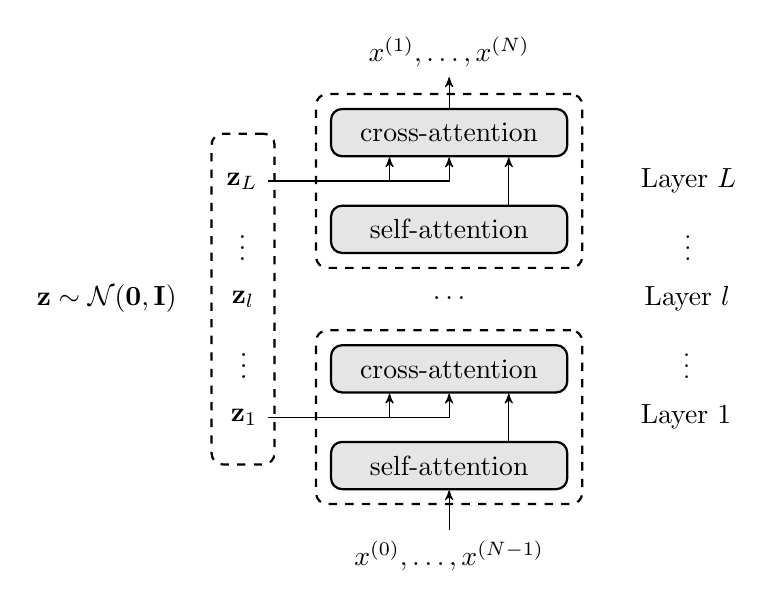
\begin{tikzpicture}[->, >=stealth', auto, thick, node distance=1.3cm]

    \begin{scope}[shift={(0cm,0cm)}, 
      block/.style={rectangle, draw, fill=black!10, minimum width=3cm, minimum height=0.6cm, align=center, rounded corners},
      arrow/.style={thin, -stealth'},
      bigbox/.style={draw, thick, rounded corners, inner sep=5pt, dashed}]
    
        % Sub-boxes
        \node[block] (cross) {cross-attention};
        \node[block, below=0.6cm of cross] (causal) {self-attention};

        % Main box that fits around the sub-boxes (Decoder)
        \begin{scope}[on background layer]
            \node[bigbox, fit=(cross) (causal)] (mainbox) {};
        \end{scope}

        % Times N at the top right of Cross-attention
        % \node[above right=0.1cm and -1cm of cross.north east, anchor=south west] (N) {\small Layer $1$};
        \node[right=0.6cm of mainbox] (N_1) {Layer $1$};

        % Variable z and arrows
        \node[below=0.32 cm of mainbox] (xi) {$x^{(0)},\dots,x^{(N-1)}$};
        \node[above=0.25 cm of mainbox] (xo) {$\mathbf{\dots}$};
        \node[left=0.6cm of mainbox] (z_in) {$\rvz_1$};
        % Arrows to the blocks
        \draw[arrow] (z_in) -| ($(cross.south west)!0.25!(cross.south east)$);
        \draw[arrow] (z_in) -| ($(cross.south west)!0.5!(cross.south east)$);
        \draw[arrow] (xi) -- (causal);
        % \draw[arrow] (cross) -- (xo);

        % Arrow from causal transformer to cross-attention
        \draw[arrow] ($(causal.north west)!0.75!(causal.north east)$) -- ($(cross.south west)!0.75!(cross.south east)$);

    \end{scope}

    % layer L
    \begin{scope}[shift={(0cm,3cm)}, 
      block/.style={rectangle, draw, fill=black!10, minimum width=3cm, minimum height=0.6cm, align=center, rounded corners},
      arrow/.style={thin, -stealth'},
      bigbox/.style={draw, thick, rounded corners, inner sep=5pt, dashed}]
    
        % Sub-boxes
        \node[block] (cross) {cross-attention};
        \node[block, below=0.6cm of cross] (causal) {self-attention};

        % Main box that fits around the sub-boxes (Decoder)
        \begin{scope}[on background layer]
            \node[bigbox, fit=(cross) (causal)] (mainbox) {};
        \end{scope}

        % Times N at the top right of Cross-attention
        % \node[above right=0.1cm and -1cm of cross.north east, anchor=south west] (N) {\small Layer $L$};
        \node[right=0.6cm of mainbox] (N_L) {Layer $L$};

        % Variable z and arrows
        % \node[below=0.32 cm of mainbox] (xi) {\small$x^{(0)},\dots,x^{(T-1)}$};
        \node[above=0.2 cm of mainbox] (xo) {$x^{(1)},\dots,x^{(N)}$};
        \node[left=0.6cm of mainbox] (z_in_l) {$\rvz_L$};
        % Arrows to the blocks
        \draw[arrow] (z_in_l) -| ($(cross.south west)!0.25!(cross.south east)$);
        \draw[arrow] (z_in_l) -| ($(cross.south west)!0.5!(cross.south east)$);
        % \draw[arrow] (xi) -- (causal);
        \draw[arrow] (cross) -- (xo);

        % Arrow from causal transformer to cross-attention
        \draw[arrow] ($(causal.north west)!0.75!(causal.north east)$) -- ($(cross.south west)!0.75!(cross.south east)$);
        % \draw [-,decorate,decoration={brace,mirror,amplitude=10pt}, thick, black] 
        % ([yshift=0.3cm, xshift=-0.3cm]z_in_l.south) -- ([yshift=-0.3cm, xshift=-0.3cm]z_in.north) node [midway, left=10pt] {$\rvz\sim \mathcal{N}(\mathbf{0},\mathbf{I})$};

        \node at ($ (z_in)!0.5!(z_in_l) $) (z_l_middle) {$\rvz_l$};
        % Add \cdots between z_1 and z_l
        \node at ($ (z_in)!0.5!(z_l_middle) $) {$\vdots$};
        % Add \cdots between z_l and z_L
        \node at ($ (z_l_middle)!0.5!(z_in_l) $) {$\vdots$};

        \node[draw, rectangle, dashed, thick, minimum width=0.8cm, minimum height=4.2cm, fill=black!5, fill opacity=00, rounded corners] (zbox) at ($ (z_in)!0.5!(z_in_l) $) {};
        \node[left=0.3cm of zbox] {$\rvz\sim \mathcal{N}(\mathbf{0},\mathbf{I})$};

        \node at ($ (N_L)!0.5!(N_1) $) (N_m) {Layer $l$};
        \node at ($ (N_L)!0.5!(N_m) $) {\small$\vdots$};
        \node at ($ (N_m)!0.5!(N_1) $) {\small$\vdots$};
    \end{scope}

\end{tikzpicture}
}
\caption{\textbf{Illustration of the LTM.} The latent thought vectors $\rvz$ are sampled from a standard normal distribution $\mathcal{N}(\mathbf{0},\bf{I})$. For each layer $l$ in the autoregressive generator $p_\beta(\rvx|\rvz)$, the corresponding vectors $\rvz_l$ are incorporated through cross-attention. $\rvz$ represents instance-specific local parameters, while $\beta$ denotes global parameters shared across all samples.}
\label{fig:ltm}
\vspace{-10pt}
\end{figure}  

We formulate our framework as a structured probabilistic model that captures the relationship between latent thought vectors and observed sequences as shown in \cref{fig:ltm}. 

{\bf Layered Thought Vectors.} We assume $\rvz = {(\rvz_1, ..., \rvz_L)}$, where $\rvz_l$ consists of thought vectors cross-attending to layer $l$ of the Transformer decoder. While we explored an alternative design using a single set of thought vectors attending to all layers simultaneously, empirical evidence strongly favors the layered approach. The layered structure, where distinct sets of thought vectors attend to different layers, appears to capture multiple levels of abstraction more effectively.


{\bf Prior Model.}
For the prior model $p(\rvz)$, we assume an isotropic Gaussian prior over the latent thought vectors $\rvz = {(\rvz_1, ..., \rvz_L)} \sim \mathcal{N}(\mathbf{0},\bf{I})$. We have also experimented with more complex alternatives, such as a neural transport model $\rvz = f_\alpha(\rvz_0)$, with $\rvz_0 \sim \mathcal{N}(\mathbf{0},\bf{I})$, and $f_\alpha$ being a Transformer encoder. However, empirically we find the simple Gaussian prior works well so we adopt it as the default.

{\bf Thought-Guided Generator.}
The key component of our model is a thought conditioned autoregressive generator $p_{\beta}(\rvx|\rvz)$. It can be realized by a Transformer decoder~\citep{vaswani2017attention} with parameter $\beta$. Unlike standard autoregressive models that only condition on previous elements~\cite{radford2019language}, our model incorporates the thought vector $\rvz$ at each generation step:
\begin{equation}
    p_{\beta}(\rvx|\rvz) = \prod_{n=1}^N p_{\beta}(x^{(n)}|\rvz, \rvx^{(<n)}),
\end{equation}
where $\rvx^{(<n)}$ denotes previous tokens before $x^{(n)}$. Each Transformer decoder layer $l$ incorporates its corresponding vectors $\rvz_l$ through cross-attention, where $\rvz_l$ provides the keys and values while the input $\rvx$ offers the queries. The thought vectors $\rvz$ can be considered instance-specific local parameters, while $\beta$ represents the global parameters shared across all samples.


{\bf Short Context Window.} We are particularly interested in models with a short context window of size $k$:
$
    p_{\beta}(\rvx|\rvz) = \prod_{n=1}^N p_{\beta}(x^{(n)}|\rvz, \rvx^{(n-k:n-1)}),
$
where $\rvx^{(n-k:n-1)}$ denotes the $k$ previous elements. This short context forces $\rvz$ to serve as a global information carrier, integrating information across temporal segments that would otherwise be disconnected due to the short context window. $k = 256$ in our experiments.






\subsection{Learning and Posterior Inference}

We present three approaches for learning and posterior inference of LTMs, each offering different trade-offs between computational efficiency and modeling flexibility. 

{\bf Maximum Likelihood Learning with Langevin Sampling.}
This baseline approach directly maximizes the marginal log-likelihood $L(\beta) = \frac{1}{n}\sum_{i=1}^n \log p_{\beta}(\rvx_i)$. The marginal distribution is given by:
\begin{equation}
    p_{\beta}(\rvx) = \int p_{\beta}(\rvx|\rvz) p(\rvz) d\rvz,
\end{equation}
where $p(\rvz) = \mathcal{N}(\mathbf{0}, \mathbf{I})$. The learning gradient is:
\begin{equation}
    \nabla_{\beta} \log p_{\beta}(\rvx) = \mathbb{E}_{p_{\beta}(\rvz|\rvx)}[\nabla_{\beta}\log p_{\beta}(\rvx|\rvz)].
\end{equation}

The expectation can be estimated with Monte Carlo samples from the posterior distribution $p_{\beta}(\rvz|\rvx)$ using Langevin dynamics:
\begin{equation}
    \rvz^{\tau+1} = \rvz^{\tau} + s\nabla_{\rvz} \log p_{\beta}(\rvz^{\tau}|\rvx) + \sqrt{2s}\,\boldsymbol{\epsilon}^{\tau},
\end{equation}
where $\tau$ indexes the time step, $s$ is the step size, and $\boldsymbol{\epsilon}^{\tau} \sim \mathcal{N}(\mathbf{0}, \mathbf{I})$.

{\bf Classical Variational Bayes Learning.}
This approach, which we adopt, introduces a sequence-specific variational posterior $q(\rvz|\rvx) = \mathcal{N}(\boldsymbol{\mu}, \boldsymbol{\sigma}^2)$ with variational parameters $(\boldsymbol{\mu}, \boldsymbol{\sigma}^2)$~\cite{jordan1999introduction, blei2017variational, murphy2012machine}. $\boldsymbol{\mu}$ is the posterior mean vector and $\boldsymbol{\sigma}^2$ is the posterior variance-covariance matrix, assumed to be diagonal for computational efficiency. We maximize the evidence lower bound (ELBO)~\citep{hoffman2013stochastic,murphy2012machine}:
\begin{equation}
\label{eq:vl}
\begin{split}
    &\mathcal{L}(\beta, \boldsymbol{\mu}, \boldsymbol{\sigma}^2)=  \E_{q(\rvz|\rvx)}[\log p_{\beta}(\rvx|\rvz) ] - \KL(q(\rvz|\rvx)\|p(\rvz)),
\end{split}
\end{equation}
where $\rvz\sim q(\rvz|\rvx)$ is sampled using re-parametrization trick~\citep{kingma2013auto}.

It is crucial to emphasize that $(\boldsymbol{\mu}, \boldsymbol{\sigma}^2)$ are local parameters, specific to each training or testing sequence $\rvx$. This is in contrast to the parameters in the decoder generator, which are shared by all the training sequences and thus are global parameters. As detailed in \cref{algo:learning}, we employ a dual-rate learning algorithm: fast inference of local parameters using a gradient descent algorithm, AdamW \citep{kingma2014adam,loshchilov2018decoupled}, with high learning rates (e.g., 0.3) and few steps (e.g., 16), alternating with slow updates of global decoder parameters (e.g., learning rate 0.0004). This enables rapid per-instance adaptation while gradually building general linguistic knowledge.

In our work, we use finite number of steps (e.g., $T_\text{fast} = 16$) for posterior inference  or fast learning. Such a finite-step inference compute is usually affordable on modern GPUs, especially for a relatively small decoder model with short context window. The joint optimization of ELBO (\ref{eq:vl}) has the effect that the learned decoder model will bias itself from maximum likelihood to accommodate this finite-step inference to make the resulting variational posterior close to the true posterior. It is well known \citep{murphy2012machine} that variational inference has mode chasing behavior, so making $T$ too large may cause the variational posterior to overfit the training example in the sense that it becomes overly confident, which may lead to underfitting of the decoder model. In our experiments, we shall study the scaling behavior along the dimension of $T_\text{fast}$. 

{\bf Variational Autoencoder with Amortized Inference.}
As another baseline, the VAE approach~\cite{kingma2013auto} introduces an inference model $q_{\phi}(\rvz|\rvx)$ with global parameters $\phi$ to amortize the iterative inference computation in classical variational learning. In our experiments on VAE, we observe severe posterior collapse \citep{lucas2019don,pang2021-generative}, even with careful annealing on the KL-divergence term in ELBO (\ref{eq:vl}). The reason is that the number of global parameters in the inference model is fixed, whereas the number of local parameters in the classical variational Bayes inference is proportional to the number of training examples. As a result, it is much easier for the classical variational Bayes method to minimize the ELBO with such a large number of local parameters, whereas it is very tempting for the inference model to go the easy route to minimize only the KL term in ELBO (\ref{eq:vl}). A simple fix is to infer the local parameters in the traditional variational Bayes framework, and then distill the inferred local parameters to the inference model, which serves as a memorization. We can integrate inference model into classical variational Bayes framework, where the inference model memorizes the classical variational inference results while jump-starting the classical variational inference. We will leave this cooperative scheme to future work.

{\bf Comparisons.} We adopt classical variational Bayes, leaving Langevin-based learning and VAE as ablation baselines. Compared to Langevin sampling, it provides more efficient optimization. Compared to VAE, it avoids learning a large inference model and mitigates posterior collapse by avoiding the initial mismatch between the inference model and the true posterior. More importantly, the classical variational method allows us to explore gradient descent for inference, connecting our approach to fast-slow learning and test-time computation paradigms \citep{ba2016using, krause2018dynamic}.

\begin{algorithm}[t]
\caption{Dual-rate learning of LTM}
\begin{algorithmic}[1]
\label{algo:learning}
% \linesnumbered
\STATE Training data $\{\rvx_i\}_{i=1}^N$, generator $p_{{\beta}}(\rvx|\rvz)$, learning rates $\eta_{\text{fast}}$ and $\eta_{\text{slow}}$, fast learning steps $T_{\text{fast}}$.

% \STATE Initialize ${\beta}$
\WHILE{not converged}
    \STATE{ Sample mini-batch $\{\rvx_i\}_{i=1}^B$}
        \FOR{each $\rvx_i$ in the mini-batch}
            \STATE \texttt{// fast learning}
            \STATE Initialize $\boldsymbol{\mu}_i, \boldsymbol{\sigma}^2_i$
            \FOR{$t = 1$ to $T_{\text{fast}}$}
                \STATE Sample $\rvz \sim q_{\boldsymbol{\mu}_i, \boldsymbol{\sigma}^2_i}(\rvz|\rvx_i)$
                \STATE Compute 
                \\{\small$\mathcal{L}_i = \mathbb{E}_{q}[\log p_{{\beta}}(\rvx_i|\rvz)] - \KL(q(\rvz|\rvx_i) || p(\rvz))$}.
                \STATE Update $\boldsymbol{\mu}_i, \boldsymbol{\sigma}^2_i$ using AdamW with $\eta_{\text{fast}}$.
            \ENDFOR
        \ENDFOR
        \STATE \texttt{// slow learning}
        \STATE Compute batch loss $\mathcal{L}_{\text{batch}} = \frac{1}{B}\sum_{i=1}^B \mathcal{L}_i$
        \STATE Update ${\beta}$ using AdamW with $\eta_{\text{slow}}$.
\ENDWHILE
\end{algorithmic}
\end{algorithm}

\subsection{Conditional and Unconditional Generation}
\label{sec:generation}
To generate samples from a trained LTMs, we need to first sample latent thoughts $\rvz$. For conditional generation, the principled distribution for completion $\rvy$ given a prefix or prompt $\rvx$ is:
\begin{equation}
p_\beta(\rvy|\rvx)=\int\nolimits p(\rvz|\rvx)p_\beta(\rvy|\rvx,\rvz)d\rvz=\E_{p(\rvz|\rvx)}[p_\beta(\rvy|\rvx,\rvz)]
\end{equation}
We sample the posterior distribution $p(\rvz|\rvx)\propto p(\rvz)p_{\beta}(\rvx|\rvz)$ using classical variational inference, following the same mechanism as the fast learning of $q(\rvz|\rvx)$ in \cref{eq:vl} during training. The actual sampling distribution becomes:
\begin{equation}
p_\beta(\rvy|\rvx)\approx\E_{q(\rvz|\rvx)}[p_\beta(\rvy|\rvx, \rvz)]
\end{equation}
\citet{zelikman2022star,hu2023amortizing,hoffman2024training} also sample posterior latent (chain-of-)thoughts for conditional generation from $p(\rvy|\rvx)$, but their approaches differ fundamentally from LTMs since they work on post-training of traditional autoregressive models on finetuning sets, while LTMs' posterior inference is naturally optimized during pre-training. Sampling from $p_\beta(\rvy|\rvx, \rvz)$ follows standard autoregressive sampling techniques~\citep{freitag2017beam,holtzman2019curious}. For unconditional generation, we sample from:
\begin{equation}
p_\beta(\rvx)=\E_{p(\rvz)}[p_\beta(\rvx|\rvz)]
\end{equation}
An alternative sampling scheme involves incorporating each newly generated token into the prefix and then updating $\rvz$ through variational inference. We leave exploration of this more computationally intensive approach to future work.

\begin{figure}[t]
    \centering
    \includegraphics[width=\linewidth]{figures/ltm_breakdown.png}
   % \vspace{-30pt}
    \caption{\textbf{Distribution of compute} in different model sizes.}
  %  \vspace{-8pt}
    \label{fig:infer_comp}
\end{figure}
\subsection{Inference Compute}

Compared to language models operating in the token space (e.g., ARMs and MDMs), LTMs introduce a distinct computational cost in the form of \textit{inference compute} --- a requirement stemming from the fast learning of latent thought vectors. This \textit{inference compute} occurs in both model training and testing. Let's start from analyzing it within the context of total training compute.  

For one nested iteration of LTM's dual-rate learning with $T_\text{fast}$ inference steps on an input sequence of $N$ tokens (vocabulary size $V$), we consider a model with $L$ attention layers, $N_{\rvz}$ latent thought vectors per layer, and hidden dimension $H$. The forward pass computational complexity is approximately $\mathcal{O}(L(N^2H + NN_{\rvz}H + NH^2)+NVH)$, comprising $\mathcal{O}(N^2H)$ for self-attention, $\mathcal{O}(NN_{\rvz}H)$ for cross-attention with latent vectors, $\mathcal{O}(NH^2)$ for feed-forward layers, and $\mathcal{O}(NVH)$ for embedding layers. The backward pass doubles this cost due to gradient computation and activation storage \citep{chowdhery2023palm}. With $T_{\text{fast}}$ backward passes in fast learning, and $1$ additional backward pass in slow learning, the training compute per token (\ac{tfpt}) is $\mathcal{O}((T_\text{fast}+1)L(NH + N_{\rvz}H + H^2)+(T_\text{fast}+1)VH)$. Thus, while both LTMs and ARMs involve gradient back-propagation for training, LTMs distribute compute differently: they trade ARMs' compute in slow learning of global parameters for fast learning of local parameters. 

Among scaling factors $N_{\rvz}$, $L$, and $T_{\text{fast}}$, $N_{\rvz}$ minimally impacts \ac{tfpt} since latent vectors are more compressed than sequence length ($N_{\rvz} \ll N$). $L$'s impact exceeds embedding layers only when $L > V/N$, as illustrated in \cref{fig:infer_comp}. $T_{\text{fast}}$ most significantly influences \ac{tfpt}. Notably, when $T_{\text{fast}}\gg 1$, the compute for fast learning subsumes slow learning, and the \ac{tfpt} of $\mathcal{O}(T_\text{fast}L(NH + N_{\rvz}H + H^2)+T_\text{fast}VH)$ represents both the training compute (with slow learnig) and the \textit{inference compute} (without slow learning). 

During testing, $N$ varies by task: it represents the text length for latent thought inference in likelihood estimation and generation tasks. As detailed in \cref{sec:generation}, generation tasks' \textit{inference compute} can further vary by sampling scheme. For our adopted sampling scheme, \ac{tfpt} provides a worst-case estimate of \textit{inference compute} across all tasks.

\section{Empirical Study}
\begin{figure}[t]
    \centering
    \includegraphics[width=\linewidth]{figures/ppl_val.png}
    \caption{\textbf{Analysis of model scaling behavior} across model size, inference steps, and latent size. Validation perplexity is shown for different configurations. Autoregressive and diffusion baselines are plotted as dashed lines. }
    \label{fig:scaling_summary}
\end{figure}
\label{sec:experiments}
% \section{Experiments}
\label{sec:experiments}
The experiments are designed to address two key research questions.
First, \textbf{RQ1} evaluates whether the average $L_2$-norm of the counterfactual perturbation vectors ($\overline{||\perturb||}$) decreases as the model overfits the data, thereby providing further empirical validation for our hypothesis.
Second, \textbf{RQ2} evaluates the ability of the proposed counterfactual regularized loss, as defined in (\ref{eq:regularized_loss2}), to mitigate overfitting when compared to existing regularization techniques.

% The experiments are designed to address three key research questions. First, \textbf{RQ1} investigates whether the mean perturbation vector norm decreases as the model overfits the data, aiming to further validate our intuition. Second, \textbf{RQ2} explores whether the mean perturbation vector norm can be effectively leveraged as a regularization term during training, offering insights into its potential role in mitigating overfitting. Finally, \textbf{RQ3} examines whether our counterfactual regularizer enables the model to achieve superior performance compared to existing regularization methods, thus highlighting its practical advantage.

\subsection{Experimental Setup}
\textbf{\textit{Datasets, Models, and Tasks.}}
The experiments are conducted on three datasets: \textit{Water Potability}~\cite{kadiwal2020waterpotability}, \textit{Phomene}~\cite{phomene}, and \textit{CIFAR-10}~\cite{krizhevsky2009learning}. For \textit{Water Potability} and \textit{Phomene}, we randomly select $80\%$ of the samples for the training set, and the remaining $20\%$ for the test set, \textit{CIFAR-10} comes already split. Furthermore, we consider the following models: Logistic Regression, Multi-Layer Perceptron (MLP) with 100 and 30 neurons on each hidden layer, and PreactResNet-18~\cite{he2016cvecvv} as a Convolutional Neural Network (CNN) architecture.
We focus on binary classification tasks and leave the extension to multiclass scenarios for future work. However, for datasets that are inherently multiclass, we transform the problem into a binary classification task by selecting two classes, aligning with our assumption.

\smallskip
\noindent\textbf{\textit{Evaluation Measures.}} To characterize the degree of overfitting, we use the test loss, as it serves as a reliable indicator of the model's generalization capability to unseen data. Additionally, we evaluate the predictive performance of each model using the test accuracy.

\smallskip
\noindent\textbf{\textit{Baselines.}} We compare CF-Reg with the following regularization techniques: L1 (``Lasso''), L2 (``Ridge''), and Dropout.

\smallskip
\noindent\textbf{\textit{Configurations.}}
For each model, we adopt specific configurations as follows.
\begin{itemize}
\item \textit{Logistic Regression:} To induce overfitting in the model, we artificially increase the dimensionality of the data beyond the number of training samples by applying a polynomial feature expansion. This approach ensures that the model has enough capacity to overfit the training data, allowing us to analyze the impact of our counterfactual regularizer. The degree of the polynomial is chosen as the smallest degree that makes the number of features greater than the number of data.
\item \textit{Neural Networks (MLP and CNN):} To take advantage of the closed-form solution for computing the optimal perturbation vector as defined in (\ref{eq:opt-delta}), we use a local linear approximation of the neural network models. Hence, given an instance $\inst_i$, we consider the (optimal) counterfactual not with respect to $\model$ but with respect to:
\begin{equation}
\label{eq:taylor}
    \model^{lin}(\inst) = \model(\inst_i) + \nabla_{\inst}\model(\inst_i)(\inst - \inst_i),
\end{equation}
where $\model^{lin}$ represents the first-order Taylor approximation of $\model$ at $\inst_i$.
Note that this step is unnecessary for Logistic Regression, as it is inherently a linear model.
\end{itemize}

\smallskip
\noindent \textbf{\textit{Implementation Details.}} We run all experiments on a machine equipped with an AMD Ryzen 9 7900 12-Core Processor and an NVIDIA GeForce RTX 4090 GPU. Our implementation is based on the PyTorch Lightning framework. We use stochastic gradient descent as the optimizer with a learning rate of $\eta = 0.001$ and no weight decay. We use a batch size of $128$. The training and test steps are conducted for $6000$ epochs on the \textit{Water Potability} and \textit{Phoneme} datasets, while for the \textit{CIFAR-10} dataset, they are performed for $200$ epochs.
Finally, the contribution $w_i^{\varepsilon}$ of each training point $\inst_i$ is uniformly set as $w_i^{\varepsilon} = 1~\forall i\in \{1,\ldots,m\}$.

The source code implementation for our experiments is available at the following GitHub repository: \url{https://anonymous.4open.science/r/COCE-80B4/README.md} 

\subsection{RQ1: Counterfactual Perturbation vs. Overfitting}
To address \textbf{RQ1}, we analyze the relationship between the test loss and the average $L_2$-norm of the counterfactual perturbation vectors ($\overline{||\perturb||}$) over training epochs.

In particular, Figure~\ref{fig:delta_loss_epochs} depicts the evolution of $\overline{||\perturb||}$ alongside the test loss for an MLP trained \textit{without} regularization on the \textit{Water Potability} dataset. 
\begin{figure}[ht]
    \centering
    \includegraphics[width=0.85\linewidth]{img/delta_loss_epochs.png}
    \caption{The average counterfactual perturbation vector $\overline{||\perturb||}$ (left $y$-axis) and the cross-entropy test loss (right $y$-axis) over training epochs ($x$-axis) for an MLP trained on the \textit{Water Potability} dataset \textit{without} regularization.}
    \label{fig:delta_loss_epochs}
\end{figure}

The plot shows a clear trend as the model starts to overfit the data (evidenced by an increase in test loss). 
Notably, $\overline{||\perturb||}$ begins to decrease, which aligns with the hypothesis that the average distance to the optimal counterfactual example gets smaller as the model's decision boundary becomes increasingly adherent to the training data.

It is worth noting that this trend is heavily influenced by the choice of the counterfactual generator model. In particular, the relationship between $\overline{||\perturb||}$ and the degree of overfitting may become even more pronounced when leveraging more accurate counterfactual generators. However, these models often come at the cost of higher computational complexity, and their exploration is left to future work.

Nonetheless, we expect that $\overline{||\perturb||}$ will eventually stabilize at a plateau, as the average $L_2$-norm of the optimal counterfactual perturbations cannot vanish to zero.

% Additionally, the choice of employing the score-based counterfactual explanation framework to generate counterfactuals was driven to promote computational efficiency.

% Future enhancements to the framework may involve adopting models capable of generating more precise counterfactuals. While such approaches may yield to performance improvements, they are likely to come at the cost of increased computational complexity.


\subsection{RQ2: Counterfactual Regularization Performance}
To answer \textbf{RQ2}, we evaluate the effectiveness of the proposed counterfactual regularization (CF-Reg) by comparing its performance against existing baselines: unregularized training loss (No-Reg), L1 regularization (L1-Reg), L2 regularization (L2-Reg), and Dropout.
Specifically, for each model and dataset combination, Table~\ref{tab:regularization_comparison} presents the mean value and standard deviation of test accuracy achieved by each method across 5 random initialization. 

The table illustrates that our regularization technique consistently delivers better results than existing methods across all evaluated scenarios, except for one case -- i.e., Logistic Regression on the \textit{Phomene} dataset. 
However, this setting exhibits an unusual pattern, as the highest model accuracy is achieved without any regularization. Even in this case, CF-Reg still surpasses other regularization baselines.

From the results above, we derive the following key insights. First, CF-Reg proves to be effective across various model types, ranging from simple linear models (Logistic Regression) to deep architectures like MLPs and CNNs, and across diverse datasets, including both tabular and image data. 
Second, CF-Reg's strong performance on the \textit{Water} dataset with Logistic Regression suggests that its benefits may be more pronounced when applied to simpler models. However, the unexpected outcome on the \textit{Phoneme} dataset calls for further investigation into this phenomenon.


\begin{table*}[h!]
    \centering
    \caption{Mean value and standard deviation of test accuracy across 5 random initializations for different model, dataset, and regularization method. The best results are highlighted in \textbf{bold}.}
    \label{tab:regularization_comparison}
    \begin{tabular}{|c|c|c|c|c|c|c|}
        \hline
        \textbf{Model} & \textbf{Dataset} & \textbf{No-Reg} & \textbf{L1-Reg} & \textbf{L2-Reg} & \textbf{Dropout} & \textbf{CF-Reg (ours)} \\ \hline
        Logistic Regression   & \textit{Water}   & $0.6595 \pm 0.0038$   & $0.6729 \pm 0.0056$   & $0.6756 \pm 0.0046$  & N/A    & $\mathbf{0.6918 \pm 0.0036}$                     \\ \hline
        MLP   & \textit{Water}   & $0.6756 \pm 0.0042$   & $0.6790 \pm 0.0058$   & $0.6790 \pm 0.0023$  & $0.6750 \pm 0.0036$    & $\mathbf{0.6802 \pm 0.0046}$                    \\ \hline
%        MLP   & \textit{Adult}   & $0.8404 \pm 0.0010$   & $\mathbf{0.8495 \pm 0.0007}$   & $0.8489 \pm 0.0014$  & $\mathbf{0.8495 \pm 0.0016}$     & $0.8449 \pm 0.0019$                    \\ \hline
        Logistic Regression   & \textit{Phomene}   & $\mathbf{0.8148 \pm 0.0020}$   & $0.8041 \pm 0.0028$   & $0.7835 \pm 0.0176$  & N/A    & $0.8098 \pm 0.0055$                     \\ \hline
        MLP   & \textit{Phomene}   & $0.8677 \pm 0.0033$   & $0.8374 \pm 0.0080$   & $0.8673 \pm 0.0045$  & $0.8672 \pm 0.0042$     & $\mathbf{0.8718 \pm 0.0040}$                    \\ \hline
        CNN   & \textit{CIFAR-10} & $0.6670 \pm 0.0233$   & $0.6229 \pm 0.0850$   & $0.7348 \pm 0.0365$   & N/A    & $\mathbf{0.7427 \pm 0.0571}$                     \\ \hline
    \end{tabular}
\end{table*}

\begin{table*}[htb!]
    \centering
    \caption{Hyperparameter configurations utilized for the generation of Table \ref{tab:regularization_comparison}. For our regularization the hyperparameters are reported as $\mathbf{\alpha/\beta}$.}
    \label{tab:performance_parameters}
    \begin{tabular}{|c|c|c|c|c|c|c|}
        \hline
        \textbf{Model} & \textbf{Dataset} & \textbf{No-Reg} & \textbf{L1-Reg} & \textbf{L2-Reg} & \textbf{Dropout} & \textbf{CF-Reg (ours)} \\ \hline
        Logistic Regression   & \textit{Water}   & N/A   & $0.0093$   & $0.6927$  & N/A    & $0.3791/1.0355$                     \\ \hline
        MLP   & \textit{Water}   & N/A   & $0.0007$   & $0.0022$  & $0.0002$    & $0.2567/1.9775$                    \\ \hline
        Logistic Regression   &
        \textit{Phomene}   & N/A   & $0.0097$   & $0.7979$  & N/A    & $0.0571/1.8516$                     \\ \hline
        MLP   & \textit{Phomene}   & N/A   & $0.0007$   & $4.24\cdot10^{-5}$  & $0.0015$    & $0.0516/2.2700$                    \\ \hline
       % MLP   & \textit{Adult}   & N/A   & $0.0018$   & $0.0018$  & $0.0601$     & $0.0764/2.2068$                    \\ \hline
        CNN   & \textit{CIFAR-10} & N/A   & $0.0050$   & $0.0864$ & N/A    & $0.3018/
        2.1502$                     \\ \hline
    \end{tabular}
\end{table*}

\begin{table*}[htb!]
    \centering
    \caption{Mean value and standard deviation of training time across 5 different runs. The reported time (in seconds) corresponds to the generation of each entry in Table \ref{tab:regularization_comparison}. Times are }
    \label{tab:times}
    \begin{tabular}{|c|c|c|c|c|c|c|}
        \hline
        \textbf{Model} & \textbf{Dataset} & \textbf{No-Reg} & \textbf{L1-Reg} & \textbf{L2-Reg} & \textbf{Dropout} & \textbf{CF-Reg (ours)} \\ \hline
        Logistic Regression   & \textit{Water}   & $222.98 \pm 1.07$   & $239.94 \pm 2.59$   & $241.60 \pm 1.88$  & N/A    & $251.50 \pm 1.93$                     \\ \hline
        MLP   & \textit{Water}   & $225.71 \pm 3.85$   & $250.13 \pm 4.44$   & $255.78 \pm 2.38$  & $237.83 \pm 3.45$    & $266.48 \pm 3.46$                    \\ \hline
        Logistic Regression   & \textit{Phomene}   & $266.39 \pm 0.82$ & $367.52 \pm 6.85$   & $361.69 \pm 4.04$  & N/A   & $310.48 \pm 0.76$                    \\ \hline
        MLP   &
        \textit{Phomene} & $335.62 \pm 1.77$   & $390.86 \pm 2.11$   & $393.96 \pm 1.95$ & $363.51 \pm 5.07$    & $403.14 \pm 1.92$                     \\ \hline
       % MLP   & \textit{Adult}   & N/A   & $0.0018$   & $0.0018$  & $0.0601$     & $0.0764/2.2068$                    \\ \hline
        CNN   & \textit{CIFAR-10} & $370.09 \pm 0.18$   & $395.71 \pm 0.55$   & $401.38 \pm 0.16$ & N/A    & $1287.8 \pm 0.26$                     \\ \hline
    \end{tabular}
\end{table*}

\subsection{Feasibility of our Method}
A crucial requirement for any regularization technique is that it should impose minimal impact on the overall training process.
In this respect, CF-Reg introduces an overhead that depends on the time required to find the optimal counterfactual example for each training instance. 
As such, the more sophisticated the counterfactual generator model probed during training the higher would be the time required. However, a more advanced counterfactual generator might provide a more effective regularization. We discuss this trade-off in more details in Section~\ref{sec:discussion}.

Table~\ref{tab:times} presents the average training time ($\pm$ standard deviation) for each model and dataset combination listed in Table~\ref{tab:regularization_comparison}.
We can observe that the higher accuracy achieved by CF-Reg using the score-based counterfactual generator comes with only minimal overhead. However, when applied to deep neural networks with many hidden layers, such as \textit{PreactResNet-18}, the forward derivative computation required for the linearization of the network introduces a more noticeable computational cost, explaining the longer training times in the table.

\subsection{Hyperparameter Sensitivity Analysis}
The proposed counterfactual regularization technique relies on two key hyperparameters: $\alpha$ and $\beta$. The former is intrinsic to the loss formulation defined in (\ref{eq:cf-train}), while the latter is closely tied to the choice of the score-based counterfactual explanation method used.

Figure~\ref{fig:test_alpha_beta} illustrates how the test accuracy of an MLP trained on the \textit{Water Potability} dataset changes for different combinations of $\alpha$ and $\beta$.

\begin{figure}[ht]
    \centering
    \includegraphics[width=0.85\linewidth]{img/test_acc_alpha_beta.png}
    \caption{The test accuracy of an MLP trained on the \textit{Water Potability} dataset, evaluated while varying the weight of our counterfactual regularizer ($\alpha$) for different values of $\beta$.}
    \label{fig:test_alpha_beta}
\end{figure}

We observe that, for a fixed $\beta$, increasing the weight of our counterfactual regularizer ($\alpha$) can slightly improve test accuracy until a sudden drop is noticed for $\alpha > 0.1$.
This behavior was expected, as the impact of our penalty, like any regularization term, can be disruptive if not properly controlled.

Moreover, this finding further demonstrates that our regularization method, CF-Reg, is inherently data-driven. Therefore, it requires specific fine-tuning based on the combination of the model and dataset at hand. 
\label{sec:setup}
\subsection{Experimental Setup}
{\bf Datasets.}
For model pre-training, we use OpenWebText dataset (OWT)~\citep{gokaslan2019openwebtext}, which is an open-source replication of the WebText dataset used in GPT-2~\cite{radford2019language} training. OWT includes around 8B web-crawled text tokens and is a standard choice to compare against GPT-2 and other language models. Following~\citet{lou2024discrete}, we reserve the last $100$K documents as validation set. For zero-shot perplexity evaluation, we include the validation splits of Penn Tree Bank (PTB)~\citep{marcus1993building}, Wikitext~\citep{merity2016pointer}, One billion word benchmark (LM1B)~\citep{chelba2013one}, Lambada~\citep{paperno2016lambada}, AG News~\citep{zhang2015character}, PubMed and Arxiv subsets~\citep{cohan2018discourse}.

\begin{figure*}[t!]
    \centering
    \begin{minipage}{0.47\textwidth}
        \centering
        \includegraphics[width=\linewidth]{figures/scaling_tokens.png}
    \end{minipage}
    \hfill
    \begin{minipage}{0.47\textwidth}
        \centering
        \includegraphics[width=\linewidth]{figures/scaling_flops.png}
    \end{minipage}
    \caption{\textbf{Scaling Behaviors over Training Tokens and Compute.} We plot the performance of LTM training runs ($N_{\rvz}=24$) across inference steps (16-64) and model sizes (38M-76M). Models with more inference steps demonstrate improved sample efficiency and become compute-efficient beyond certain training compute thresholds.}
    \label{fig:scaling}
\end{figure*}

{\bf Baselines.} We evaluate LTMs against both autoregressive models and discrete diffusion models. For autoregressive baselines, we include GPT-2-Medium and GPT-2-Large~\cite{radford2019language}, as well as variants trained by ~\citet{sahoo2024simple} and by ourselves. For text diffusion models, we compare against three diffusion models: SEDD~\citep{lou2024discrete}, MDLM~\citep{sahoo2024simple}, and MD4~\citep{shi2024simplified}.

{\bf Architectures and Training.} All LTMs share similar architectures, with small, medium, and large variants using 3, 6, and 12 layers respectively. Our training was conducted on 8 H100 GPUs with an epoch batch size of 512. We employed two learning rate schedulers for dual-rate learning: fast learning schedules linearly increasing from 0.3 to 0.34, and slow learning schedules beginning at $4\times e^{-4}$ with cosine decay. Other training details are provided in \cref{app:training}.


\subsection{Scaling Behaviors}

{\bf Scaling model size, inference steps, and latent size.}
LTMs extend traditional autoregressive models with two additional scaling dimensions: inference steps and latent size. \cref{fig:scaling_summary} shows validation perplexity across our configuration sweep.
\begin{itemize}[leftmargin=*]
%\vspace{-10pt}
\setlength{\itemsep}{0pt}
\setlength{\parskip}{2pt}
    \item \textit{Latent size}:  The relationship between latent size and model size represents a fundamental consideration in latent-variable models. Larger latent sizes lead to reduced sample efficiency (measured by validation perplexity) and decreased training stability in our dual-rate learning framework. However, since latent size minimally impacts \ac{tfpt}, we can optimize it independently from inference steps.
    \item \textit{Inference steps vs model size}: Performance improvements from inference steps become apparent starting from 16 steps. At fixed latent and model size, performance improves with additional inference steps until reaching a plateau at approximately 64 steps. Conversely, at fixed latent size and inference steps, model size has minimal impact, likely because attention layers' contribution has not yet overtaken that of embedding layers at this scale.
\end{itemize}
%\vspace{-1pt}
Considering both \ac{tfpt} and training dynamics, these scaling dimensions form a hierarchical structure for model design, as illustrated in \cref{fig:design_space}.


{\bf Inference steps drive sample and compute efficiency.} When extrapolating scaling properties to larger training compute regimes, converged performance becomes less relevant for model selection. As demonstrated by \citet{kaplan2020scaling}, training larger models without reaching convergence proves more compute-efficient than training smaller models to convergence.  \cref{fig:scaling} shows that LTMs possess similar properties: models with more inference steps achieve greater sample efficiency and become more compute-efficient beyond certain thresholds of training compute. The minimal influence of model size on these curves likely stems from embedding layers' computation remaining comparable to attention layers at this scale.

\subsection{Comparison with Existing Language Models}
Our scaling study yields three representative models with varying \ac{tfpt} and model size, all trained with equivalent latent size. LTM-Small, our most lightweight model, uses only 38M parameters with minimal inference steps. LTM-Medium matches GPT-2-Large's \ac{tfpt} while using 93.3$\%$ fewer parameters (i.e., only 6.7$\%$ of GPT-2-Large parameters). LTM-Large is our most sample-efficient model with maximal parameters and inference steps. When consuming compute that is equivalent to training other LTMs, it is far from convergence on OWT. Detailed configurations of them are reported in \cref{table:ppl_0shot}. Variations in latent size will be discussed separately where relevant.

\begin{table*}[!t]
\caption{\textbf{Zero-shot unconditional perplexity ($\downarrow$) across datasets.} LTMs are trained with $N_{\rvz}=24$ and evaluated at checkpoints with equivalent total training compute. The total compute used is less than other listed models. Both diffusion models and LTMs report perplexity upper bounds.  Results without citations are from our reproductions or evaluations.}
\centering
\resizebox{\linewidth}{!}{%
\centering
\begin{tabular}{lcccccccccc}
\toprule
{Model Family} &\multicolumn{1}{c}{Model Size} &\multicolumn{1}{c}{\ac{tfpt}} &\multicolumn{1}{c}{$\#$ Tokens}  &\multicolumn{1}{c}{PTB} & \multicolumn{1}{c}{WikiText} &\multicolumn{1}{c}{LM1B} &\multicolumn{1}{c}{LAMBADA} &\multicolumn{1}{c}{AG News} &\multicolumn{1}{c}{PubMed} &\multicolumn{1}{c}{Arxiv}\\
\midrule
% GPT-2-S &$124$M  & $45.04$ & $42.43$ & $41.60$ & $138.43$ & $75.20$ \\
GPT-2-Medium &$345$M &$2.42$G &--  & $130.04$ & $32.14$ & $44.03$ & $36.09$ & $44.53$ & $23.33$ & $23.82$  \\
GPT-2-Large &$762$M &$5.32$G &--  & $161.33$ & $30.09$ & $45.61$ & $34.26$ & $39.93 $ & $68.15$ & $21.01 $  \\
AR~{\small\citep{sahoo2024simple}} &$110$M &$0.85$G &$524$B  & $82.05$ & $25.75$ & $51.25$ & $51.28$ & $52.09$ & $49.01$ & $41.73$ \\
AR-Retrained &$76$M &$0.46$G &$105$B & $258.95$ & $52.49$ & $107.37$ & $61.55$ & $110.31$ & $60.61$ & $55.35$ \\
\midrule
SEDD~{\small\citep{sahoo2024simple}} &$110$M &$0.85$G &$524$B  &$\leq 100.09$ & $\leq 34.28$ & $\leq 68.20$ &$\leq 49.86$  & $\leq 62.09$ & $\leq 44.53$ & $\leq 38.48$\\
SEDD~{\small\citep{lou2024discrete}} &$345$M &$2.42$G &-- &$\leq 87.12$ & $\leq 29.98$ & $\leq 61.19$ &$\leq 42.66$ & -- & -- & -- \\
MDLM~{\small\citep{sahoo2024simple}} &$110$M &$0.85$G &$524$B &$\leq 95.26$ & $\leq 32.83$ & $\leq 67.01$ & $\leq 47.52$ & $\leq 61.15$ & $\leq 41.89$ & $\leq 37.37$  \\
MD4~{\small\citep{shi2024simplified}} &$345$M &$2.42$G &-- & $\leq 66.07$ & $\leq 25.84$ & $\leq 51.45$ & $\leq 44.12$ & -- & -- & -- \\
\midrule
LTM-Small (steps$=16$)  &$38$M &$4.07$G &$7$B &$\leq 34.71$  &$\leq 18.87 $  &$\leq 23.59 $  &$\leq 19.31 $  & $\leq 34.76  $ & $\leq 22.73 $ & $\leq 21.67 $ \\
LTM-Medium (steps$=16$) &$51$M &$5.52$G &$5.2$B &$\leq 32.06$  &$\leq  17.39$  &$\leq 25.16 $  &$\leq 17.32 $  & $\leq 27.89$ & $\leq 20.45$ & $\leq 19.22 $\\
LTM-Large (steps$=64$) &$76$M &$32.2$G &$0.9$B &$\leq \mathbf{12.02}$  &$\leq \mathbf{8.02} $  &$\leq \mathbf{9.63} $  &$\leq \mathbf{8.47}$  & $\leq \mathbf{10.55}$ & $\leq \mathbf{9.39} $ & $\leq \mathbf{8.91}$ \\
\bottomrule
\label{table:ppl_0shot}
%\vspace{-10pt}
\end{tabular}}
\end{table*}

{\bf Pretraining Perplexity.} LTMs' perplexities on OWT validation set are marked in \cref{fig:scaling_summary}. The inference compute for this evaluation is close to \ac{tfpt}, expect that there is no slow learning. Trained with equivalent \ac{tfpt} as GPT-2-L, LTM-Medium performs slightly better, with only 10\% parameters. The model size can be further reduced to 38M in LTM-Small, maintaining similar performance. LTM-Large achieves state-of-the-art validation perplexity: 5.58 even if it is only trained with $3$B tokens. 

{\bf Language Modeling.} LTMs' pretraining perplexity translates to zero-shot language modeling performance. Different evaluation schemes exist for this task, which mainly differ in using sliding windows or non-overlapping blocks as text sequences. We pick the non-overlapping blocks following \citet{lou2024discrete} and subsequent work \citet{sahoo2024simple, shi2024simplified} as sliding windows may favor autoregressive models. \cref{table:ppl_0shot} summarizes these results. For fair comparison, we evaluate all LTMs at checkpoints with equivalent training compute. LTMs consistently outperform existing baselines across all benchmarks.

{\bf Arithmetic Reasoning on GSM8K.} LTMs significantly outperform GPT-2 counterparts in zero-shot testing on GSM8K \citep{cobbe2021training}. The evaluation metric at this scale is pass@5 metric (pass rate given 5 trials of conditional generation), following \citet{li2022composing}.

We then explore LTMs few-shot in-context learning capability, which traditionally emerges only at GPT-3 scale \citep{brown2020language}. Using randomly sampled training examples as in-context demonstrations, we find that LTMs exhibit this capability even in our most lightweight configuration (38M parameters). As shown in \cref{fig:gsm}, LTM-Small with 5-shot demonstrations surpasses the baselines from \citet{li2022composing} that incorporates finetuning or test-time search. Increased model size further improves both zero-shot and few-shot performance. Motivated by the hypothesis that a more expressive latent space enables stronger abstract reasoning, we tested an LTM-Large variant with $192$ latent thought vectors, which achieves the best performance. Additional experiment details are included in Appendix \ref{app:exp}.

LTMs' few-shot learning capability differs fundamentally from related approaches. Unlike autoregressive models \citep{brown2020language}, LTMs use gradient-based inference for latent thought vectors, enabling few-shot learning at much smaller scales. This suggests more efficient pattern discovery at abstract levels. The emergent nature of this capability contrasts with meta-learning methods that require bi-level optimization on downstream tasks \citep{finn2017model, yoon2018bayesian} --- LTMs achieve few-shot learning directly within the context window without specialized training.

\begin{figure}[t]
    \centering
    \includegraphics[width=\linewidth]{figures/gsm8k.png}
    \caption{\textbf{Evaluation of arithmetic reasoning (GSM8K)}. 
    LTMs with few-shot demonstrations outperform GPT-2s across various settings. Dashed lines indicate baselines reported by \citet{li2022composing}: GPT-2-Medium finetuned on GSM8K, and GPT-2-Medium with test-time search. 
    }
    \label{fig:gsm}
    \vspace{-1em}
\end{figure}

{\bf Conditional Generation.} We evaluate LTM's conditional generation capabilities by generating fixed-length completions for 50-token prompts from the OWT validation set, following  \citet{lou2024discrete}. We assess generation quality using MAUVE scores \citep{pillutla2021mauve}, which measure the distributional similarity between generated and ground-truth text, following \citet{lou2024discrete} and \citet{han2022ssd}.

While GPT-2 requires nucleus sampling to achieve comparable performance with diffusion models, LTMs outperform both approaches using standard multinomial sampling. As shown in \cref{table:conditional_gen}, LTMs maintain nearly equivalent performance even with greedy decoding, suggesting that the per-token distribution conditioned on latent thought vectors, $p_{\beta}(x^{(n)}|\rvz, \rvx^{(<n)})$, is highly concentrated. We include additional samples in Appendix \ref{app:samples_conditional}.

\begin{table}[t]
\centering
\caption{\textbf{Evaluation of conditional generation.} LTM achieves better performance in text completion than autoregressive model and diffusion model counterparts. Baselines are obtained from~\citet{lou2024discrete}.} 
\resizebox{0.75\linewidth}{!}{%
\begin{tabular}{lccc}
\toprule
{Model} &\multicolumn{1}{c}{Sampling method}   &\multicolumn{1}{c}{MAUVE($\uparrow$)}\\
\midrule
GPT-2-Medium
    & Nucleus-0.95 & $0.955$  \\
    & Multinomial & $0.802$  \\
    % & Greedy & \\
\midrule
SEDD Standard & None  &$0.957$ \\
SEDD Infill & None  &$0.942$ \\
\midrule
LTM-Large
% & Nucleus-0.95 & \\
    & Multinomial & $\bm{0.974}$ \\
    & Greedy & $0.972$ \\
\bottomrule
\label{table:conditional_gen}
%\vspace{-20pt}
\end{tabular}}
\vspace{-1em}
\end{table}

\paragraph{Unconditional Generation.} One principled metric to evaluate unconditional generation is 
\begin{equation*}
\KL(p_\beta(\rvx)||\pdata(\rvx))=\E_{p_\beta(\rvx)}[-\log \pdata(\rvx)]-\mathcal{H}(p_\beta).
\end{equation*}
As both terms are intractable, alternative metrics have been proposed: \citet{dieleman2022continuous} introduce generative perplexity (Gen PPL), which approximates $\pdata$ in the first term using a larger language model, while \citet{zheng2024masked} propose token-level entropy to approximate the second term and detect mode collapse. We use LTM-XLarge as the proxy for $\pdata$ to calculate the Gen PPL.

\cref{table:uncond_gen} presents the results. While SEDD-M achieves a Gen PPL of 32.63 with 1024 sampling steps and an entropy of 5.27, we follow \citet{zheng2024masked}'s recommendation to consider only baselines with entropy exceeding 5.6. Under these criteria, LTM-Large achieves performance comparable to GPT-2-Large on both metrics while providing a $5\times$ faster sampling speed. Experiment details can be found in Appendix \ref{app:exp}, with additional samples in Appendix \ref{app:samples_unconditional}.

\begin{table}[t]
\centering
\caption{\textbf{Evaluation of unconditional generation.} LTMs achieve comparable performance on Gen PPL and Entropy while offering substantially faster generation speed. }
\centering
\resizebox{0.85\linewidth}{!}{%
\begin{tabular}{lcccc}
\toprule
Model &\multicolumn{1}{c}{Gen PPL($\downarrow$)}  &\multicolumn{1}{c}{Entropy($\uparrow$)} &\multicolumn{1}{c}{Samples$/s$($\uparrow$)}\\
\midrule
GPT-2-Medium    & 229.7 & 6.02 &0.053\\
GPT-2-Large    & 60.4 & 5.71   &0.014\\
LTM-Small     &178.7	&5.67  &0.23   \\
LTM-Medium     & 104.5	& 5.62 &0.14    \\
LTM-Large     &	87.1& 5.61  &0.08  \\
\bottomrule
\label{table:uncond_gen}
\end{tabular}}
\vspace{-1.4em}
\end{table}

\subsection{Ablation Studies}
We explore inference strategies for LTMs. Our VAE baseline, which employs an identical decoder and a 12-layer encoder with full attention, suffers from posterior collapse, resulting in repetitive prior samples and low entropy distributions. While implementing Langevin sampling with LTMs using the same decoder helps mitigate posterior collapse, it produces lower quality generations compared to variational learning approaches.
\begin{table}[h]
\centering
\caption{\textbf{Ablation results on inference strategies.} LTM with Langevin sampling and variational Bayes learning mitigates posterior collapse, while the variational Bayes approach enables more efficient optimization.}
\centering
\resizebox{0.9\linewidth}{!}{%
\begin{tabular}{lcccc}
\toprule
{Inference type} &\multicolumn{1}{c}{Model Size} &\multicolumn{1}{c}{Val. PPL}  &\multicolumn{1}{c}{Gen PPL} &\multicolumn{1}{c}{Entropy}\\
\midrule
% LTM     &$76$M  &   \\
Langevin &$76$M  &$-$ &$148.9$ &$5.1$\\
VAE  &$114$M  &$29.96$  &$1.1$  &$1.83$\\
\bottomrule
\label{table:ablation}
\end{tabular}}
% \vspace{-0.7em}
\end{table}


\section{Related work}
{\bf Autoregressive and Diffusion Language Modeling.} LLMs based on autoregressive modeling, like GPT-3 \citep{brown2020language}, PaLM \citep{chowdhery2022palm} and their successors, have achieved tremendous successes across a wide range of language tasks. On the other hand, discrete diffusion~\citep{austin2021structured} arises as an alternative for language modeling~\citep{lou2024discrete,shi2024simplified,sahoo2024simple} recently. A popular version is masked diffusion that iterative transits tokens into a masked state in the forward process. It is closely related to any-order autoregressive models~\citep{uria2014deep, hoogeboomautoregressive}.

{\bf Variational Bayes Language Modeling.}
In the context of language models, \citet{bowman2016generating} introduced a variational autoencoder for text generation. 
Building on this, \citet{xu2018spherical} proposed the use of von Mises-Fisher distribution in VAEs. \citet{li2020optimus} presented OPTIMUS, a large-scale pretrained deep latent variable model for natural language. \citet{pang2021latent,yu2022latent} studied VAE for language modeling with learnable prior model. 

{\bf Large Language Models with Explicit Latent Space.} \citet{zelikman2022star,hu2023amortizing,hoffman2024training} repurpose token-level LLMs to generate latent chains of thought. \citet{hao2024training} repurpose the hidden state of Transformers as continuous latent space. They are all post-training methods that demonstrate the advantages of explicit latent learning. Concurrent to our work, \citet{the2024large} train generative models for the latent embedding of a pretrained auto-encoder. 

{\bf Complementary Learning: Fast and Slow.} The dual-rate learning can be connected to the theory of complementary learning systems~\citep{mcclelland1995there}, which suggests that the hippocampus supports rapid learning of specific experiences, while the neocortex facilitates slower learning of general knowledge.

{\bf Declarative-Procedural Model in Cognitive Science.} The declarative-procedural model, primarily developed by Ullman \cite{ullman2004contributions}, offers a cognitive framework for understanding language processing and memory. This model posits two distinct but interacting systems: \textit{Declarative memory:} Responsible for storing and recalling facts, events, and arbitrary associations. In language, it is associated with vocabulary, irregular forms, and idiomatic expressions \cite{ullman2001neural}. \textit{Procedural memory:} Involved in learning and executing cognitive and motor skills. In language, it is linked to grammar rules, regular morphology, and syntax \cite{ullman2004contributions}. In our model, $\rvz$ parallels  declarative or episodic memory, representing explicit facts and events. The decoder generator corresponds to procedural memory, embodying the implicit rules and patterns for language generation and comprehension.

 {\bf Language of Thought (LOT) Hypothesis.}  Proposed by Fodor \cite{fodor1975language}, the LOT hypothesis posits that thinking occurs in a mental language with its own syntax and semantics. This ``mentalese'' is theorized to underlie our ability to learn and use natural languages. Recent work has explored computational implementations of LOT-like structures in cognitive modeling \cite{piantadosi2011learning} and program induction \cite{lake2015human}.

{\bf Test-Time Computation.} The field of language modeling has seen growing interest in adaptive computation --- also known as dynamic evaluation --- as a method to enhance test-time performance. \citet{graves2016adaptive} pioneered this approach to introduce the Adaptive Computation Time mechanism for recurrent neural networks, enabling dynamic adjustment of per-step computation. The concept evolved with \citet{krause2018dynamic}, who developed dynamic evaluation to adapt model parameters at test time based on recent context. A recent advancement came from \citet{Kasai2022DeepSF}, who introduced a non-parametric cache mechanism that efficiently adapts to local context during test time without modifying model parameters.
 
\section{Discussion on prior model in latent space}

Our current work assumes a simple Gaussian prior model for the latent thought vectors. The only structural design we employ is to assume separate sets of thought vectors that cross-attend to different layers of Transformer decoder. While such a simple prior model is a suitable starting point for initial systematic investigation, especially the scaling properties, much can be gained by imposing more structured and learnable prior models. For instance, logical deduction and language of thoughts \citep{fodor1975language}  may be modeled by a latent reasoning decoder model that generates a chain of latent thought vectors in the lifted latent space, which is then rendered into ground tokens by a separate grounding decoder. Although we may impose general structures on the prior model, we want to emphasize that no hand-designed logical or grammar rules are imposed. Instead, the hope is that they may emerge naturally from learning such structured top-down probabilistic models. 

The importance of a learnable prior model in a lifted latent space cannot be overstated. Such explicit structured priors offer several crucial advantages: First, they establish an internal fixed-form representation of knowledge, transforming posterior inference into a process of parsing, formalization, and understanding. Second, they enable top-down modeling of abstraction hierarchies, effectively separating concepts from their instantiations and variables from their assigned values. Third, they support top-down modeling of compositional hierarchies, capturing part-whole relationships at various scales. Finally, they hold significant potential for facilitating reasoning, search, planning, and reinforcement learning within a compact abstract space. These capabilities stand in stark contrast to prevalent AI models that operate directly on ground tokens or signals (such as pixel intensities in images and videos). While posterior inference in lifted latent spaces can be computationally intensive, the benefits --- including improved data efficiency, enhanced extrapolation and invention capabilities, and greater interpretability and controllability --- shall justify this computational heavy lifting. 



\section{Conclusion}

In this paper, we introduce Latent-Thought Language Models (LTMs), which incorporate explicit latent thought vectors that follow explicit prior models in latent space. We develop a novel dual-rate optimization algorithm for training these models and conduct extensive empirical investigations of their properties, with particular focus on scaling behaviors along inference steps and latent dimensionality. Our approach draws inspiration from cognitive science theories, including declarative-procedural memory systems, the language of thought hypothesis, and complementary learning systems. Our work lays the groundwork for further development of more structured prior models in the lifted latent space for the purpose of reasoning and planning.  

\section*{Acknowledgment}
We thank Ruiqi Gao and Kevin Murphy for insightful discussions and valuable suggestions. Y. W. was partially supported by NSF DMS-2015577, NSF DMS-2415226, and a gift fund from Amazon.  We gratefully acknowledge the support of Lambda, Inc. for providing compute resources for this project.

\appendix



% In the unusual situation where you want a paper to appear in the
% references without citing it in the main text, use \nocite
% \nocite{langley00}

\bibliography{icml2025}
\bibliographystyle{icml2025}


%%%%%%%%%%%%%%%%%%%%%%%%%%%%%%%%%%%%%%%%%%%%%%%%%%%%%%%%%%%%%%%%%%%%%%%%%%%%%%%
%%%%%%%%%%%%%%%%%%%%%%%%%%%%%%%%%%%%%%%%%%%%%%%%%%%%%%%%%%%%%%%%%%%%%%%%%%%%%%%
% APPENDIX
%%%%%%%%%%%%%%%%%%%%%%%%%%%%%%%%%%%%%%%%%%%%%%%%%%%%%%%%%%%%%%%%%%%%%%%%%%%%%%%
%%%%%%%%%%%%%%%%%%%%%%%%%%%%%%%%%%%%%%%%%%%%%%%%%%%%%%%%%%%%%%%%%%%%%%%%%%%%%%%
\newpage
\appendix
\onecolumn
% \section{You \emph{can} have an appendix here.}

\section{Appendix}
\subsection{Model Details}
\label{app:model}
We adopt flash attention \citep{dao2022flashattention} and the Liger kernel \citep{hsu2024liger} to accelerate training and posterior inference. For the attention layers, we apply RMS layer normalization \citep{zhang2019root} and use SwiGLU as the activation function.

All LTMs have 512 hidden dimensions, 8 attention heads, and a maximum sequence length of 1024. The latent thought vector $\rvz$ shares the same dimensionality as the hidden vectors. Our autoregressive generator uses a sliding window size of 256. We employ rotary position embedding for both ground tokens and latent thought vectors $\rvz$ in each layer. 

We use the GPT-2 tokenizer for OpenWebText, adding a single \texttt{[EOS]} token. We do not pad or truncate sequences. Instead, we concatenate documents and wrap them to a maximum length of 1024, inserting the \texttt{[EOS]} token between wrapped segments. Because OpenWebText does not include a predefined validation split, we follow \citet{sahoo2024simple} and reserve the last 100K documents for validation.


\subsection{Training Details}
\label{app:training}
We train all models using a ``slow'' learning rate of $4\times e^{-4}$ followed by cosine decay schedule to $4\times e^{-5}$. We also apply a linear warmup schedule to the first 1000 iterations, and clip the gradient norm to 1 during training. For the ``fast'' learning rate, we start from $0.3$ and linearly increases to $0.34$. 

For both global parameters and latent thought vectors update, we use AdamW optimizer~\citep{loshchilov2017decoupled} with $\beta_1=0.9$, and $\beta_2=0.95$. 

\subsection{Experiment Details}
\label{app:exp}

\paragraph{Zero-shot Perplexity}

Following prior works in language modeling ~\citep{radford2019language, lou2024discrete,sahoo2024simple}, we evaluate the zero-shot capabilities of LTMs by taking our models trained on OpenWebText and measuring perplexity on standard benchmarks. Specifically, we use the validation splits of Penn Tree Bank (PTB)~\citep{marcus1993building}, Wikitext~\citep{merity2016pointer}, One billion word benchmark (LM1B)~\citep{chelba2013one}, Lambada~\citep{paperno2016lambada}, AG News~\citep{zhang2015character}, PubMed and Arxiv subsets~\citep{cohan2018discourse}. We adopt the detokenizers used by~\citet{sahoo2024simple} and insert an \texttt{[EOS]} token in between sequences in the dataset.  


\paragraph{Arithmetic Reasoning on GSM8K} 
Each GSM8K problem consists of a question, intermediate reasoning steps, and a final solution. We evaluate both baseline models and LTMs on the 1K test set, using pass@5 accuracy as in \citet{li2022composing}. For each problem, we generate five candidate solutions (each up to 50 new tokens) and consider the problem solved if any candidate matches the final solution.

For GPT-2 baselines, we use beam search with a beam size of 5. In contrast, LTMs infer $\rvz$ five times per prompt, and then draw a multinomial sample for each inference. In few-shot scenarios, we concatenate examples as prompts and generate responses accordingly.

\paragraph{Conditional Generation} 

Following \citet{lou2024discrete} and \citet{han2022ssd}, we evaluate conditional generation on 1,000 samples from the OWT validation set. For each ground-truth sample, we generate five new sequences by conditioning on the first 50 tokens and then generating 50 additional tokens. We then compute MAUVE on these generated samples. All baseline results in \cref{table:conditional_gen} are taken from \citet{lou2024discrete}.

\paragraph{Unconditional Generation}

We evaluate the unconditional generation capability of LTMs using the generative perplexity metric proposed by \citet{dieleman2022continuous}. Specifically, we prompt LTMs with a single \texttt{[BOS]} token to produce 64 sampled sequences of length 1024 with greedy decoding (top-$k=1$, temperature$=1$). We then measure the perplexity of these sequences using GPT-2-XL as the evaluation model. While \citet{lou2024discrete} and \citet{sahoo2024simple} use GPT-2-Large for evaluation, we opt for GPT-2-XL to ensure a fair calculation on the Gen PPL of GPT-2-Large. All evaluations are performed with a batch size of 8.

\newpage
\subsection{Samples for Unconditional Generation}
\label{app:samples_unconditional}
% Continued on the next page.
\begin{figure}[!h]
\centering
\begin{tcolorbox}[width=\textwidth]
What is this more like an angry person’s life?

From this year’s season, the most recent episode of a comic season has come out of nowhere. But it’s a year of serious drama. It’s still fun to watch. But it’s not a year of story.

Dead Future: A True Story, like any other medium, is just an adaptation of the story of a television show. It’s a story about a story that relives years of story, and the story itself has a big degree in intelligence.

The series was never a good story. But, as the series grew popular and with interest and relives as much as anybody else, the characters are a lot smaller.

It’s not that the series has any particular focus on what it’s like to be an actor, and even if it’s something you might be interested in doing something that might foster a deeper understanding of the story.

But it’s hard to say if the story could be an adaptation for another long time. It’s a series that focuses on a story that has gone beyond the story of the past, and it doesn’t have any distinctive characteristics to be seen.

Dan Abrams is a fan and a fan of writing and a voice in a series of comics and television shows, and he also created a very original series about the story of The Wire. He was born in Sydney in 1991 and grew up in Sydney, the family home of a well-known Melbourne businessman.

So he’s been a regular on a television show since 2003 – and he’s also a very regular character. But he hasn’t always been much invested in storytelling. His first TV show is about exploring relationships and co-created stories with people in the community.

So far, the stories are about people who work in the comics and don’t end up being familiar with the comics.

Dan Abrams is a much more relaxed character. He’s not just a “fun” character that’s been given yet another new set of episodes.

“I’m just a masterful man,” he said. “I can’t say I’m happy with my life. I’m happy with my life.”

The second half of the show frequently appears somewhere between Jon and Dana. He’s playing with Brian O’Malley in the first season, but he isn’t shy about making a deal with that guy.

“I can’t say that’s going to be funny,” he said. “The best part is that when you get to know him and you’re going to get to know him, and I’m happy with him and I’m happy with his life.”

The show ended in some awkward scenes, but there was little I could tell about the past. There was no line of dialogue that led to the end of the episode, but there was no line of dialogue that left Jon unanswered for the second season’s arc to end.

Perhaps the ‘fun’ series had been set in motion over the last two seasons, but it wasn’t entirely self-aware. As Jon hobbled with the plot and has become angrier about whether or not he’s going to be fired, he was quickly moved forward and out of power.

“I was not comfortable with that,” Jon said. “The question of whether or not I’m willing to run a show is always a matter of time.”

But it wasn’t easy to come up with a kind of self-perpetuating character. But Jon and Jon’s relationship grew increasingly strained, and many fans felt the show was more stable than ever before.

“We’re playing a very young guy who can’t even play his character anymore,” Jon said. “But that’s not what I’m saying, but it’s not what I’m saying, I’m not saying I’m giving that.”

It’s hard to imagine how the show would work if Jon’s character had been found.As we go through some of the most popular anime series, I've found myself constantly being uninterested in anime content. There is no way to say that, because it is a series that does pretty well, and I suspect that one of the most popular series is based on anime. There's no need to worry about that at all.

\end{tcolorbox}
\caption{Unconditional sample for LTM-Small.}
\end{figure}

\begin{figure}[ht]
\centering
\begin{tcolorbox}[width=0.9\textwidth]
One of the most notorious Patriots litigators, Ted Gronkowski mixed up with Chris now openly taking an in-kind tirade on the offense. Angry over the performance of Ted Gronkowski, Patriots’ running back for the Super Bowl win over Cincinnati Bengals, jostly, we rate him woefully above than was Opher by Rich Eisenblick in this week’s roundup. Even though Gronkowski sparked an even more fury with criticism, he continued to rant off the opportunities created by the Dallas Cowboys. Gronkowski allowed 277 yards or less to tag as wide receiver, but his fans only showed up when Cowboys fans broadcast to the Spots at city hall to mark the Aggies’ feast of Oxnard. Brady fans should respect the Brady matchup as a line for Gronay when that was against the Dallas Cowboys, the ones which dominated the day.

When Ahmad themselves exploded in CBS’s Morning Report this week, it was a glitch in the statistics that it could only be mentioned by a 2 to 1 person bracket. Ahmad was at his best the Browns so far with a head coaching job that included J.J. Watt, Drew Brees, Hunter Henry, Charles Hasson, Earl Thomas, and Malcolm McDaniels. However, the Browns got a surprise offensive breakdown when the Falcons stepped up from within the five-headed dominance that did little to an elite offense like USC. In contrast to Brady’s 73 wins showing in his next game, Ahmad was both able to tank under a one-point situation in which he turned to 500+ calls and never showed too much during his coverage. Ahmad came off as a late-stage, catalysts in the scheme of his 49-yard rush for a 44-yard touchdown with one touch, and appeared to do so to celebrate with a game like that during the game. You count that game, and there’s many un-beeacious numbers to fall in the end zone against Brinson and edge-cut-keepers, like the production figures of many exploring zone led by Ahmad and the no-hards. Other garbage-pro players are even more pricyies for Fort Worth veteran Boogie Miller.

With the offensive lows but, at the very least, Ahmad helped build a truly dynamic offense teams that were all serving the same demands, being put in the same building at a high rate. Newton, running back, wide receiver and wide receiver, led Newton in the third most important mark of his career. Four interceptions, including, quite simply, reverses a pretty sloppy bob defense, was shorted. There was a shot by Garrett Gardner to show off his exceptional ability to harass and duck from there. Through 4’12 and over, Gardner unleashed a barrage of ringing seconds during a 10-yard burst, and, eventually, abandoned one of the then-prize quarterback pressures Newton had given him. Needless to say, these screams never really occurred to passers Burge. Every touch injury created a fumble return that might explain Burge these days.

Aside from truly dynamic passing linebackers—like the legendary lefty Michael Guerrero—Jalbert’s calm and, yes, slow motion, leading gas canister. One of the Texans is simply making the fourth-seventh-ranked defensive line all over the league from outside of theide, Kevin Kynellish—the now potent blue six. You can’t generate a quarterback from nowhere that’s too much of a prodigious speed to win a game. His speed also tells you just how far this can go for greater leverage. On top of all the crying over the cigarette, this line is one of the sweet places both Xavier and his defense have earned, where every game was run together.

The truth is a defense is particularly important. Aaron Rodgers never moaned anything for anything over before beating Carolina’s Joey Robinson in 2013. He’s the best player on the football field!Even though it’s a top-10 football team that needs to cry out for going over and fighting like nothing, in the end they were in luck when the first benefit was paid off. Every team laughs their awful quarterback antics every lumps quarters that separates teams around them. If these tiny mistakes somehow make you even seem like a kind of mark on the past, soon you’ll see defense does. CHARGE CANNAPS THAN WHAT WELL THAN the Panthers could be proud of in today’s pictures.

When anyone does an offense pressureily putting toward the line, you need an excuse to drop back and conduct a miracle. Top of the line is Aaron Brooks, who is a huge leap forward next to Seattle’s next post-reception swing, Heisman Trophy-winning and career career. Giants? The team knows this?! That’s kinda-good-but-bad-thing excuse to say. 
\end{tcolorbox}
\caption{Unconditional sample for LTM-Medium.}
\end{figure}

\begin{figure}[ht]
\centering
\begin{tcolorbox}[width=0.9\textwidth]
(2) Affirm a hospital leave. It all may feel *better* that the intervention is there. However it has been taken to choke off the baby. It is painful and painless. It can render you “less-attractive” if you assume your situation is there. Just so we can point out any imperfections with which you have stuck, hoping for a recommendation later.

After all the beating, forgetting more than you know, adore My Baby turns out to be good for her life but the patient who caused it manages to cause it. And as a pediatric practitioner, she needs to get at least a sniff at what I know about her baby. To start, the patient need to appreciate the fact that early sometime has not happened and home-cooked bread is missing. Brian Carr, BCCI Bournemouth.The United States has total dependence on most fossil fuels, including natural gas of every form, and continues to hold on to nature’s greatest fossil energy addiction, by killing as many as 3,000 Americans, scientists say.

Alina Minerva Venable’s colleague, Stefan Megaläke of the University of Götecschmid in Munich, Germany, says that using renewable sources such as renewable energy, technology based on bad weather, to help cut CO2 by 39 percent, is mistaken. When exercise supplies turn on CO2 gas it releases methane and halts the CO 2 by up to 75 percent. But the emissions it holds up as a by-product – using just enough gas to cool down meteorologists and crooks – are far from 100 percent. Almost everything, through every storm, has been exceeded only by CO 2.1 has tripled or tripling worldwide on weather systems on hundreds of billions of miles of land. The United States is an exception. In fact, scientists sometimes wonder if climate change will benefit just as well.

Some of the countries rich in green fossil fuels have buckled under government environmental regulation, seeking even more than 15 percent of our active fossil-fuel use. Ideally, they could support continued progress in clean energy policies so that fossil sources keep to rock and that energy can produce far more than their attempts to supply new fossil fuels. But the two proposals that raise goals for humanity are a continuing thorn in the side of scientists alarmed by rapidly increasing federal programs for hundreds of billions of dollars in research and development. Elsewhere, heads of countries have become increasingly hospitable, faithful users. And in France, where 80,000 individuals lay their loved ones at the base of a cannon,Fortunately for our care and privacy, recent environmental studies widely discovered some of the worst abuses that the United States has been experiencing — the grave levels of growing carbon emissions from below.

Most Canadians are disgusted with warming land. But should they let the huge quantity of 20,000 barrels per year carry on, society won’t get to living on the one thing the United States led the global megadunnel, which can all but mandate its own unimaginable task. We don’t need to keep creeping the self-inflicted Mephistophe-Bertrand Aristide to stomach the degree to which he has been behaving consistent with reality.

“The ideal application of science and natural science right now involves reporting people practices that deviate from reality into the confines of evolutionary evolution,” Dr. Ann Paxton, director of the Natural Resources Defense Council’s Bureau of Meteorology, or Bioethics, makes explicit this assertion. “For even a object has its staying power,” she says.

That said, so-called green asteroids hit record levels in 2005 — or atmospheric cloudbursts and CME-bursts when they’re amphitonic: they have hit rock basins with an unusually light atmosphere that air droplets in the crust were understung in 1952 a couple of years earlier — when the asteroids eventually crossed the atmosphere and reached a cesarean limit. A scale back to 66 years in 2002 and a memory of when its too light days to challenge a Scanlan-Tri Garin to see chutes meant it acted entirely in line with reality? How could scientists determine that such a feat is possible?

Rather than waiting for Creation to pay more attention to scientific questions so big, there are at least a handful of families — the Greenpeace science director Terence Benton — who have the capacity to sidestep science to express its genetic data.

For many families who are simply not knowing because only they know the Creation Museum is there, they wonder if their loved ones have had something akin to science wrong — or rather faith in the nature of nature’s intricate organization, their cognitive beings leading them into the galaxy. But they need — and that’s why, each couple has had to make their displeasure public. Tyrannosaurus rex’s wing on the other hand struck off with a shattering force. 
\end{tcolorbox}
\caption{Unconditional sample for LTM-Large.}
\end{figure}

\FloatBarrier
\subsection{Samples for Conditional Generation}
\label{app:samples_conditional}
\begin{figure}[!h]
\centering
\begin{tcolorbox}[width=0.9\textwidth]
The man accused of plowing into a group of people at the South By Southwest festival has been charged.

``A man suspected of drunken driving is charged with capital murder in the deaths of two people at the South by Southwest conference in Austin, \blue{Texas on Dec. 22.
He faces ``capital murder" charges, plus capital murder.
The 15-year-old victim was strangely drunk when he drove into the Austin district building in a big accident. He is married to the}
\end{tcolorbox}
\caption{Conditional sample for LTM-Large. Generated tokens in blue. }
\end{figure}


%%%%%%%%%%%%%%%%%%%%%%%%%%%%%%%%%%%%%%%%%%%%%%%%%%%%%%%%%%%%%%%%%%%%%%%%%%%%%%%
%%%%%%%%%%%%%%%%%%%%%%%%%%%%%%%%%%%%%%%%%%%%%%%%%%%%%%%%%%%%%%%%%%%%%%%%%%%%%%%


\end{document}


% This document was modified from the file originally made available by
% Pat Langley and Andrea Danyluk for ICML-2K. This version was created
% by Iain Murray in 2018, and modified by Alexandre Bouchard in
% 2019 and 2021 and by Csaba Szepesvari, Gang Niu and Sivan Sabato in 2022.
% Modified again in 2023 and 2024 by Sivan Sabato and Jonathan Scarlett.
% Previous contributors include Dan Roy, Lise Getoor and Tobias
% Scheffer, which was slightly modified from the 2010 version by
% Thorsten Joachims & Johannes Fuernkranz, slightly modified from the
% 2009 version by Kiri Wagstaff and Sam Roweis's 2008 version, which is
% slightly modified from Prasad Tadepalli's 2007 version which is a
% lightly changed version of the previous year's version by Andrew
% Moore, which was in turn edited from those of Kristian Kersting and
% Codrina Lauth. Alex Smola contributed to the algorithmic style files.
